\documentclass[twoside]{article}

% Packages required by doxygen
\usepackage{calc}
\usepackage{doxygen}
\usepackage{graphicx}
\usepackage[utf8]{inputenc}
\usepackage{makeidx}
\usepackage{multicol}
\usepackage{multirow}
\PassOptionsToPackage{warn}{textcomp}
\usepackage{textcomp}
\usepackage[nointegrals]{wasysym}
\usepackage[table]{xcolor}

% Font selection
\usepackage[T1]{fontenc}
\usepackage{mathptmx}
\usepackage[scaled=.90]{helvet}
\usepackage{courier}
\usepackage{amssymb}
\usepackage{sectsty}
\renewcommand{\familydefault}{\sfdefault}
\allsectionsfont{%
  \fontseries{bc}\selectfont%
  \color{darkgray}%
}
\renewcommand{\DoxyLabelFont}{%
  \fontseries{bc}\selectfont%
  \color{darkgray}%
}
\newcommand{\+}{\discretionary{\mbox{\scriptsize$\hookleftarrow$}}{}{}}

% Page & text layout
\usepackage{geometry}
\geometry{%
  a4paper,%
  top=2.5cm,%
  bottom=2.5cm,%
  left=2.5cm,%
  right=2.5cm%
}
\tolerance=750
\hfuzz=15pt
\hbadness=750
\setlength{\emergencystretch}{15pt}
\setlength{\parindent}{0cm}
\setlength{\parskip}{0.2cm}
\makeatletter
\renewcommand{\paragraph}{%
  \@startsection{paragraph}{4}{0ex}{-1.0ex}{1.0ex}{%
    \normalfont\normalsize\bfseries\SS@parafont%
  }%
}
\renewcommand{\subparagraph}{%
  \@startsection{subparagraph}{5}{0ex}{-1.0ex}{1.0ex}{%
    \normalfont\normalsize\bfseries\SS@subparafont%
  }%
}
\makeatother

% Headers & footers
\usepackage{fancyhdr}
\pagestyle{fancyplain}
\fancyhead[LE]{\fancyplain{}{\bfseries\thepage}}
\fancyhead[CE]{\fancyplain{}{}}
\fancyhead[RE]{\fancyplain{}{\bfseries\leftmark}}
\fancyhead[LO]{\fancyplain{}{\bfseries\rightmark}}
\fancyhead[CO]{\fancyplain{}{}}
\fancyhead[RO]{\fancyplain{}{\bfseries\thepage}}
\fancyfoot[LE]{\fancyplain{}{}}
\fancyfoot[CE]{\fancyplain{}{}}
\fancyfoot[RE]{\fancyplain{}{\bfseries\scriptsize Generated on Sat May 3 2014 20\+:22\+:34 for P\+B\+N Analyzer by Doxygen }}
\fancyfoot[LO]{\fancyplain{}{\bfseries\scriptsize Generated on Sat May 3 2014 20\+:22\+:34 for P\+B\+N Analyzer by Doxygen }}
\fancyfoot[CO]{\fancyplain{}{}}
\fancyfoot[RO]{\fancyplain{}{}}
\renewcommand{\footrulewidth}{0.4pt}
\renewcommand{\sectionmark}[1]{%
  \markright{\thesection\ #1}%
}

% Indices & bibliography
\usepackage{natbib}
\usepackage[titles]{tocloft}
\setcounter{tocdepth}{3}
\setcounter{secnumdepth}{5}
\makeindex

% Hyperlinks (required, but should be loaded last)
\usepackage{ifpdf}
\ifpdf
  \usepackage[pdftex,pagebackref=true]{hyperref}
\else
  \usepackage[ps2pdf,pagebackref=true]{hyperref}
\fi
\hypersetup{%
  colorlinks=true,%
  linkcolor=blue,%
  citecolor=blue,%
  unicode%
}

% Custom commands
\newcommand{\clearemptydoublepage}{%
  \newpage{\pagestyle{empty}\cleardoublepage}%
}


%===== C O N T E N T S =====

\begin{document}

% Titlepage & ToC
\hypersetup{pageanchor=false,
             bookmarks=true,
             bookmarksnumbered=true,
             pdfencoding=unicode
            }
\pagenumbering{roman}
\begin{titlepage}
\vspace*{7cm}
\begin{center}%
{\Large P\+B\+N Analyzer }\\
\vspace*{1cm}
{\large Generated by Doxygen 1.8.6}\\
\vspace*{0.5cm}
{\small Sat May 3 2014 20:22:34}\\
\end{center}
\end{titlepage}
\tableofcontents
\pagenumbering{arabic}
\hypersetup{pageanchor=true}

%--- Begin generated contents ---
\section{P\+B\+N Analyzer 2.1}
\label{index}\hypertarget{index}{}An application for Simulation/\+Inverse Decomposition of Probabilistic Boolean Networks.\hypertarget{index_Introduction}{}\subsection{Introduction}\label{index_Introduction}
This is an open-\/source application that can be used in the research/analysis of P\+B\+N systems.

For users, you can inverse decompose your own transition matrix data and get the Entropy, Decomposition and Time data, or you can simulate random boolean matrices and weights for transition matrices.

For developer users, you can test your own algorithms using this A\+P\+I. Only the inverse algorithm part has to be implemented, all other functionalities are provided by the application itself.\hypertarget{index_Compilation}{}\subsection{Compilation}\label{index_Compilation}
This application now comes with the source file with makefile and is currently a console application working on U\+N\+I\+X-\/like systems.

If you are on Mac\+O\+S or Linux System, just unzip the \char`\"{}\+Analyzer.\+zip\char`\"{} file, then use the terminal to go into \char`\"{}\+Release\char`\"{} folder, type \char`\"{}make\char`\"{} to compile the binary. Then type \char`\"{}./\+Analyzer\char`\"{} to run the application.

If you are on Windows system, you should first download and install \char`\"{}cygwin\char`\"{} with \char`\"{}gcc, make\char`\"{} packages following the website After that, put the unzipped file in your home directory where your \char`\"{}cygwin\char`\"{} executable is. Then repeat the steps for Mac\+O\+S system.\hypertarget{index_Mannual}{}\subsection{Mannual}\label{index_Mannual}
When running the Analyzer application, first a menu will pop up and user are aked to choose a funcional module.
\begin{DoxyEnumerate}
\item Simulate data \+: This module will simulate test data and save the data in directory \char`\"{}\+Input/\+Simulated\char`\"{}. It is advised to input descriptive suffix when asked for.
\item Test provided data \+: This module will let the user test their own provided data. First make sure that your matrix data is in \char`\"{}.\+txt\char`\"{} format with columns separated by \char`\"{}\+Tabs\char`\"{} and rows separated by \char`\"{}new\+Lines\char`\"{}. The application has a \char`\"{}default mode\char`\"{} where it assumes you are testing \char`\"{}\+Provided data\char`\"{} rather than \char`\"{}\+Simulated data\char`\"{} and the algorithm used will be \char`\"{}\+O\+P\+T\+I\+M\+A\+L\char`\"{}. User can configure the mode according to their own need.
\item and 4. are batch testing modules, on \char`\"{}\+Simulated data\char`\"{} and \char`\"{}\+Provided data\char`\"{} respectively. The test data are prepared and upon chosen, the module will directly start running.
\end{DoxyEnumerate}\hypertarget{index_Developer}{}\subsection{Developer}\label{index_Developer}
If you want to use the application for testing your own inverse decomposition algorithm, you should follow the steps\+: Step 1 \+: Go to \char`\"{}\+Release/config.\+txt\char`\"{} and add the name of your algorithm in a new line before \char`\"{}\+\_\+\+D\+E\+F\+A\+U\+L\+T\+\_\+\char`\"{}; Step 2 \+: Go to \char`\"{}\+Interactor.\+h\char`\"{} and add your algorithm name to the Enum \char`\"{}\+Random\+Types\char`\"{}; Step 3 \+: Here since the class responsible for doing inverse decomposition is the \char`\"{}\+Iterator\char`\"{} class, there are basically two ways to add a new algorithm. One is write a subclass of \char`\"{}\+Iterator\char`\"{} class and override the \char`\"{}\+Iterate\char`\"{} method to include your new algorithm. The second will be just modifying the original \char`\"{}\+Iterate\char`\"{} method. But for the second way you might need to check the implementation of \char`\"{}iterate\+Once\char`\"{} and \char`\"{}choose\+Entry\char`\"{} methods. Both method requires your implementation of the algorithm in as separate function.\hypertarget{index_Design}{}\subsection{Design}\label{index_Design}
The major design used in this application is the \char`\"{}\+Model-\/\+View-\/\+Controller\char`\"{} design, where the \char`\"{}\+Interactor\char`\"{} serves as the \char`\"{}\+Abstract of Controller\char`\"{}. The \char`\"{}\+View\char`\"{} part is abstracted in an interface called \char`\"{}\+Displayer\char`\"{}. When moving to other platforms or building a G\+U\+I, the most important part to rewrite is the \char`\"{}\+Menu\char`\"{} which is a subclass of \char`\"{}\+Interactor\char`\"{} that implements the \char`\"{}\+Displayer\char`\"{} interface. Hence completing the task of user interaction.

The algorithms are encapsulated in the \char`\"{}\+Model\char`\"{} part consists of \char`\"{}\+Simulator\char`\"{} and \char`\"{}\+Iterator\char`\"{}, where \char`\"{}\+Simulator\char`\"{} class is responsible for simulating transition matrix and \char`\"{}\+Iterator\char`\"{} class is responsible for doing inverse decomposition.

For further details, or usage of classes during development, please refer to the documentation of this application that follows. 
\section{Module Documentation}
\hypertarget{group__matrix}{\subsection{Basic Matrices}
\label{group__matrix}\index{Basic Matrices@{Basic Matrices}}
}


This group is the basic internal data structure of this application.  


\subsubsection*{Classes}
\begin{DoxyCompactItemize}
\item 
class \hyperlink{class_abstract_matrix}{Abstract\+Matrix}
\begin{DoxyCompactList}\small\item\em This class defines some of the basic operations we need for our matrix. \end{DoxyCompactList}\item 
class \hyperlink{classr_matrix}{r\+Matrix}
\begin{DoxyCompactList}\small\item\em This class holds the data needed for representing a boolean matrix. \end{DoxyCompactList}\item 
class \hyperlink{classt_matrix}{t\+Matrix}
\begin{DoxyCompactList}\small\item\em Internal data structure representing a matrix that has constant column sums. \end{DoxyCompactList}\end{DoxyCompactItemize}


\subsubsection{Detailed Description}
This group is the basic internal data structure of this application. 

This group is the fundamental data structures used to save/load matrices and perform necessary computations. 
\hypertarget{group___u_i}{\subsection{User Interaction}
\label{group___u_i}\index{User Interaction@{User Interaction}}
}


This group contains classes used for user interaction.  


\subsubsection*{Classes}
\begin{DoxyCompactItemize}
\item 
class \hyperlink{class_displayer_1_1_displayer_class}{Displayer\+::\+Displayer\+Class}
\begin{DoxyCompactList}\small\item\em Abstract interface for direct interation with end users. \end{DoxyCompactList}\item 
class \hyperlink{class_interactor}{Interactor}
\begin{DoxyCompactList}\small\item\em An abstract controller class that contains method prototypes or basic implementations of methods for further overriding. \end{DoxyCompactList}\item 
class \hyperlink{class_menu}{Menu}
\begin{DoxyCompactList}\small\item\em This is a concrete controller class for the application. \end{DoxyCompactList}\end{DoxyCompactItemize}


\subsubsection{Detailed Description}
This group contains classes used for user interaction. 

This group contains an interface for User Interaction and also a concrete class that implements the functionality. Upgrading or migrating to other platforms/languages need reimplementation of this class. 
\hypertarget{group___processor}{\subsection{Processor}
\label{group___processor}\index{Processor@{Processor}}
}


This group contains classes for actual processing of data, both simulation and inverse iteration.  


\subsubsection*{Classes}
\begin{DoxyCompactItemize}
\item 
class \hyperlink{class_iterator}{Iterator}
\begin{DoxyCompactList}\small\item\em This class encapsulates the functionality of an inverse iterator. \end{DoxyCompactList}\item 
class \hyperlink{class_simulator}{Simulator}
\begin{DoxyCompactList}\small\item\em This is a class that handles simulation process. \end{DoxyCompactList}\end{DoxyCompactItemize}


\subsubsection{Detailed Description}
This group contains classes for actual processing of data, both simulation and inverse iteration. 

The classes in this module are \hyperlink{class_iterator}{Iterator} and \hyperlink{class_simulator}{Simulator}, serve the purposes of backward iterations and forward simulations. The usage of these two classes follows the pattern of \char`\"{}\+Initialization-\/\+Configuration-\/\+Start\char`\"{}. In the \char`\"{}\+Initialization\char`\"{} phase, the user will be asked to input necessary parameters like \char`\"{}\+Input file name\char`\"{}, \char`\"{}\+Number of Genes\char`\"{}, \char`\"{}\+File Suffix\char`\"{}. In the \char`\"{}\+Configuration\char`\"{} phase, the user has the opportunity of configuring the processor objects to the proper state like \char`\"{}\+O\+P\+T\+I\+M\+A\+L\char`\"{} or \char`\"{}\+C\+U\+B\+I\+C\char`\"{} algorithm in the inverse problem. After that, the objects will start running, generating messages indicating their states. 
\section{Class Documentation}
\hypertarget{class_abstract_matrix}{\subsection{Abstract\+Matrix Class Reference}
\label{class_abstract_matrix}\index{Abstract\+Matrix@{Abstract\+Matrix}}
}


This class defines some of the basic operations we need for our matrix.  




{\ttfamily \#include $<$Abstract\+Matrix.\+h$>$}

Inheritance diagram for Abstract\+Matrix\+:\begin{figure}[H]
\begin{center}
\leavevmode
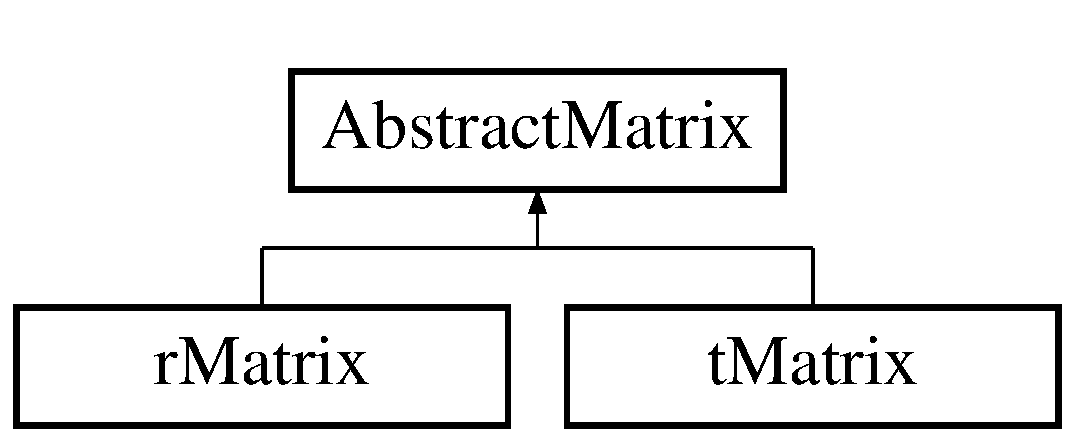
\includegraphics[height=2.000000cm]{class_abstract_matrix}
\end{center}
\end{figure}
\subsubsection*{Public Member Functions}
\begin{DoxyCompactItemize}
\item 
virtual int \hyperlink{class_abstract_matrix_a8aa21743b81e47939757beda61b33dfd}{get\+Size} () const 
\item 
virtual void \hyperlink{class_abstract_matrix_a300f90398cb2bac75c8d2ab56bdde1ab}{print} (ostream \&output)=0
\end{DoxyCompactItemize}
\subsubsection*{Protected Attributes}
\begin{DoxyCompactItemize}
\item 
int \hyperlink{class_abstract_matrix_aca80e2403cf7903a106595ba56390e99}{size}
\end{DoxyCompactItemize}


\subsubsection{Detailed Description}
This class defines some of the basic operations we need for our matrix. 

This is the basic abstract square matrix class, and all Boolean Network matrix and transition matrix should inherit from this class. 

\subsubsection{Member Function Documentation}
\hypertarget{class_abstract_matrix_a8aa21743b81e47939757beda61b33dfd}{\index{Abstract\+Matrix@{Abstract\+Matrix}!get\+Size@{get\+Size}}
\index{get\+Size@{get\+Size}!Abstract\+Matrix@{Abstract\+Matrix}}
\paragraph[{get\+Size}]{\setlength{\rightskip}{0pt plus 5cm}virtual int Abstract\+Matrix\+::get\+Size (
\begin{DoxyParamCaption}
{}
\end{DoxyParamCaption}
) const\hspace{0.3cm}{\ttfamily [virtual]}}}\label{class_abstract_matrix_a8aa21743b81e47939757beda61b33dfd}
Simple getter for the matrix, suppose the matrix is constructed with $n$ genes, then the size is $2^n$. \begin{DoxyReturn}{Returns}
The number of rows for the matrix 
\end{DoxyReturn}
\hypertarget{class_abstract_matrix_a300f90398cb2bac75c8d2ab56bdde1ab}{\index{Abstract\+Matrix@{Abstract\+Matrix}!print@{print}}
\index{print@{print}!Abstract\+Matrix@{Abstract\+Matrix}}
\paragraph[{print}]{\setlength{\rightskip}{0pt plus 5cm}virtual void Abstract\+Matrix\+::print (
\begin{DoxyParamCaption}
\item[{ostream \&}]{output}
\end{DoxyParamCaption}
)\hspace{0.3cm}{\ttfamily [pure virtual]}}}\label{class_abstract_matrix_a300f90398cb2bac75c8d2ab56bdde1ab}
Print the matrix in a n by n matrix form to the output stream 
\begin{DoxyParams}{Parameters}
{\em output} & The stream for output \\
\hline
\end{DoxyParams}


Implemented in \hyperlink{classt_matrix_a7e1b5623978bf16ace999ce22a28d350}{t\+Matrix}, and \hyperlink{classr_matrix_a2a22671198a516a8165306d5406e539b}{r\+Matrix}.



\subsubsection{Member Data Documentation}
\hypertarget{class_abstract_matrix_aca80e2403cf7903a106595ba56390e99}{\index{Abstract\+Matrix@{Abstract\+Matrix}!size@{size}}
\index{size@{size}!Abstract\+Matrix@{Abstract\+Matrix}}
\paragraph[{size}]{\setlength{\rightskip}{0pt plus 5cm}int Abstract\+Matrix\+::size\hspace{0.3cm}{\ttfamily [protected]}}}\label{class_abstract_matrix_aca80e2403cf7903a106595ba56390e99}
The size of the square matrix, inherited by its children. 

The documentation for this class was generated from the following file\+:\begin{DoxyCompactItemize}
\item 
\hyperlink{_abstract_matrix_8h}{Abstract\+Matrix.\+h}\end{DoxyCompactItemize}

\hypertarget{class_displayer_1_1_displayer_class}{\subsection{Displayer\+:\+:Displayer\+Class Class Reference}
\label{class_displayer_1_1_displayer_class}\index{Displayer\+::\+Displayer\+Class@{Displayer\+::\+Displayer\+Class}}
}


Abstract interface for direct interation with end users.  




{\ttfamily \#include $<$Displayer.\+h$>$}

Inheritance diagram for Displayer\+:\+:Displayer\+Class\+:\begin{figure}[H]
\begin{center}
\leavevmode
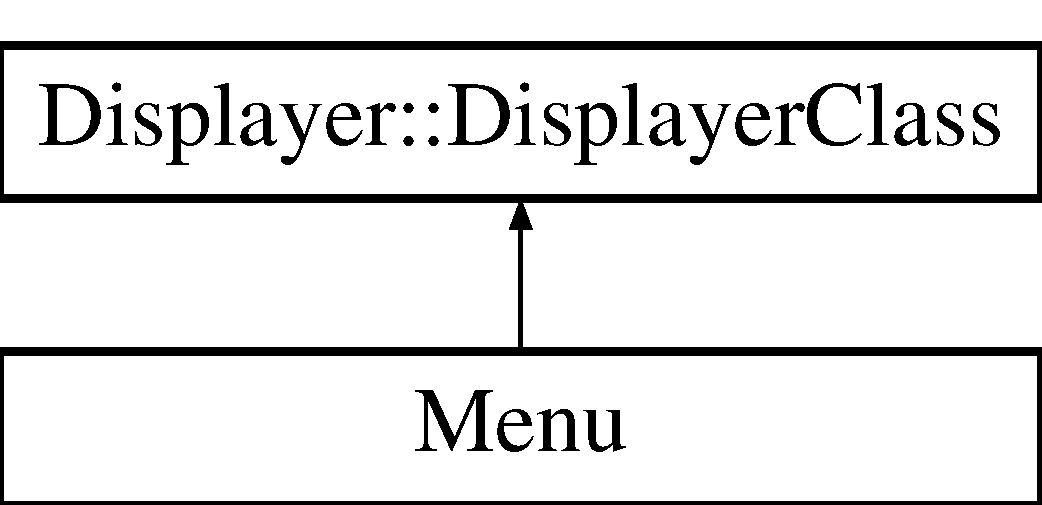
\includegraphics[height=2.000000cm]{class_displayer_1_1_displayer_class}
\end{center}
\end{figure}
\subsubsection*{Public Member Functions}
\begin{DoxyCompactItemize}
\item 
virtual void \hyperlink{class_displayer_1_1_displayer_class_aa259ca88fafe20ad118cb8a492c88351}{show\+Menu} ()=0
\item 
virtual void \hyperlink{class_displayer_1_1_displayer_class_ac61f3852eda7fe91a189927d33d4aef5}{get\+Choice} ()=0
\end{DoxyCompactItemize}
\subsubsection*{Protected Attributes}
\begin{DoxyCompactItemize}
\item 
\hypertarget{class_displayer_1_1_displayer_class_a13a8fff0d761fc68d208d5bb16429395}{char \hyperlink{class_displayer_1_1_displayer_class_a13a8fff0d761fc68d208d5bb16429395}{choice}}\label{class_displayer_1_1_displayer_class_a13a8fff0d761fc68d208d5bb16429395}

\begin{DoxyCompactList}\small\item\em A character representing the choice of users. \end{DoxyCompactList}\end{DoxyCompactItemize}
\subsubsection*{Private Member Functions}
\begin{DoxyCompactItemize}
\item 
virtual void \hyperlink{class_displayer_1_1_displayer_class_a84478e90e6895f0061268c59d2040cc4}{parse\+Choice} ()=0
\item 
virtual void \hyperlink{class_displayer_1_1_displayer_class_ae572acc400418de40d2977a7b5556d45}{display\+Message} (string message)=0
\item 
virtual void \hyperlink{class_displayer_1_1_displayer_class_a9b9ea4661b05a211763792e392f3cdd5}{check\+Matrix} (\hyperlink{classt_matrix}{t\+Matrix} $\ast$transition)=0
\item 
virtual void \hyperlink{class_displayer_1_1_displayer_class_a1ae1ffba6ab3b1effad2b042e2868ac4}{exit\+Program} ()=0
\end{DoxyCompactItemize}


\subsubsection{Detailed Description}
Abstract interface for direct interation with end users. 

This class declares function prototypes for user interactions. Any controller class should implement this interface. 

\subsubsection{Member Function Documentation}
\hypertarget{class_displayer_1_1_displayer_class_a9b9ea4661b05a211763792e392f3cdd5}{\index{Displayer\+::\+Displayer\+Class@{Displayer\+::\+Displayer\+Class}!check\+Matrix@{check\+Matrix}}
\index{check\+Matrix@{check\+Matrix}!Displayer\+::\+Displayer\+Class@{Displayer\+::\+Displayer\+Class}}
\paragraph[{check\+Matrix}]{\setlength{\rightskip}{0pt plus 5cm}virtual void Displayer\+::\+Displayer\+Class\+::check\+Matrix (
\begin{DoxyParamCaption}
\item[{{\bf t\+Matrix} $\ast$}]{transition}
\end{DoxyParamCaption}
)\hspace{0.3cm}{\ttfamily [private]}, {\ttfamily [pure virtual]}}}\label{class_displayer_1_1_displayer_class_a9b9ea4661b05a211763792e392f3cdd5}
Display the resulting matrix to end user for double-\/check. 
\begin{DoxyParams}{Parameters}
{\em transition} & A \hyperlink{classt_matrix}{t\+Matrix} instance to display \\
\hline
\end{DoxyParams}


Implemented in \hyperlink{class_menu_a3fbf0f02d6875bc41c4ee42597d99ff1}{Menu}.

\hypertarget{class_displayer_1_1_displayer_class_ae572acc400418de40d2977a7b5556d45}{\index{Displayer\+::\+Displayer\+Class@{Displayer\+::\+Displayer\+Class}!display\+Message@{display\+Message}}
\index{display\+Message@{display\+Message}!Displayer\+::\+Displayer\+Class@{Displayer\+::\+Displayer\+Class}}
\paragraph[{display\+Message}]{\setlength{\rightskip}{0pt plus 5cm}virtual void Displayer\+::\+Displayer\+Class\+::display\+Message (
\begin{DoxyParamCaption}
\item[{string}]{message}
\end{DoxyParamCaption}
)\hspace{0.3cm}{\ttfamily [private]}, {\ttfamily [pure virtual]}}}\label{class_displayer_1_1_displayer_class_ae572acc400418de40d2977a7b5556d45}
Display a message to end user. 
\begin{DoxyParams}{Parameters}
{\em message} & The message to display. \\
\hline
\end{DoxyParams}


Implemented in \hyperlink{class_menu_a616bae73f48b58a1b5629354826c30cc}{Menu}.

\hypertarget{class_displayer_1_1_displayer_class_a1ae1ffba6ab3b1effad2b042e2868ac4}{\index{Displayer\+::\+Displayer\+Class@{Displayer\+::\+Displayer\+Class}!exit\+Program@{exit\+Program}}
\index{exit\+Program@{exit\+Program}!Displayer\+::\+Displayer\+Class@{Displayer\+::\+Displayer\+Class}}
\paragraph[{exit\+Program}]{\setlength{\rightskip}{0pt plus 5cm}virtual void Displayer\+::\+Displayer\+Class\+::exit\+Program (
\begin{DoxyParamCaption}
{}
\end{DoxyParamCaption}
)\hspace{0.3cm}{\ttfamily [private]}, {\ttfamily [pure virtual]}}}\label{class_displayer_1_1_displayer_class_a1ae1ffba6ab3b1effad2b042e2868ac4}
Action taken to exit the program. Specific behaviors when exiting could be included in this method. 

Implemented in \hyperlink{class_menu_afd50901663e9f9b1210ba9ef7512c02d}{Menu}.

\hypertarget{class_displayer_1_1_displayer_class_ac61f3852eda7fe91a189927d33d4aef5}{\index{Displayer\+::\+Displayer\+Class@{Displayer\+::\+Displayer\+Class}!get\+Choice@{get\+Choice}}
\index{get\+Choice@{get\+Choice}!Displayer\+::\+Displayer\+Class@{Displayer\+::\+Displayer\+Class}}
\paragraph[{get\+Choice}]{\setlength{\rightskip}{0pt plus 5cm}virtual void Displayer\+::\+Displayer\+Class\+::get\+Choice (
\begin{DoxyParamCaption}
{}
\end{DoxyParamCaption}
)\hspace{0.3cm}{\ttfamily [pure virtual]}}}\label{class_displayer_1_1_displayer_class_ac61f3852eda7fe91a189927d33d4aef5}
Get the choice from end users. 

Implemented in \hyperlink{class_menu_a2243881fe17494a0f6fc38a9211715d6}{Menu}.

\hypertarget{class_displayer_1_1_displayer_class_a84478e90e6895f0061268c59d2040cc4}{\index{Displayer\+::\+Displayer\+Class@{Displayer\+::\+Displayer\+Class}!parse\+Choice@{parse\+Choice}}
\index{parse\+Choice@{parse\+Choice}!Displayer\+::\+Displayer\+Class@{Displayer\+::\+Displayer\+Class}}
\paragraph[{parse\+Choice}]{\setlength{\rightskip}{0pt plus 5cm}virtual void Displayer\+::\+Displayer\+Class\+::parse\+Choice (
\begin{DoxyParamCaption}
{}
\end{DoxyParamCaption}
)\hspace{0.3cm}{\ttfamily [private]}, {\ttfamily [pure virtual]}}}\label{class_displayer_1_1_displayer_class_a84478e90e6895f0061268c59d2040cc4}
A method to parse the choice from user. Deciding which mehod to call upon each choice. 

Implemented in \hyperlink{class_menu_aad01d0f840a8be08e301d24d17b00b96}{Menu}.

\hypertarget{class_displayer_1_1_displayer_class_aa259ca88fafe20ad118cb8a492c88351}{\index{Displayer\+::\+Displayer\+Class@{Displayer\+::\+Displayer\+Class}!show\+Menu@{show\+Menu}}
\index{show\+Menu@{show\+Menu}!Displayer\+::\+Displayer\+Class@{Displayer\+::\+Displayer\+Class}}
\paragraph[{show\+Menu}]{\setlength{\rightskip}{0pt plus 5cm}virtual void Displayer\+::\+Displayer\+Class\+::show\+Menu (
\begin{DoxyParamCaption}
{}
\end{DoxyParamCaption}
)\hspace{0.3cm}{\ttfamily [pure virtual]}}}\label{class_displayer_1_1_displayer_class_aa259ca88fafe20ad118cb8a492c88351}
Displaying the menu containing choices to end users. This method should be implemented differently according to different purposes. i.\+e G\+U\+I or Console. 

Implemented in \hyperlink{class_menu_ab19f32f8deac0f6c6960f04be8612067}{Menu}.



The documentation for this class was generated from the following file\+:\begin{DoxyCompactItemize}
\item 
\hyperlink{_displayer_8h}{Displayer.\+h}\end{DoxyCompactItemize}

\hypertarget{class_file_coordinator}{\subsection{File\+Coordinator Class Reference}
\label{class_file_coordinator}\index{File\+Coordinator@{File\+Coordinator}}
}


Abstract class for file manipulations.  




{\ttfamily \#include $<$File\+Coordinator.\+h$>$}

Inheritance diagram for File\+Coordinator\+:\begin{figure}[H]
\begin{center}
\leavevmode
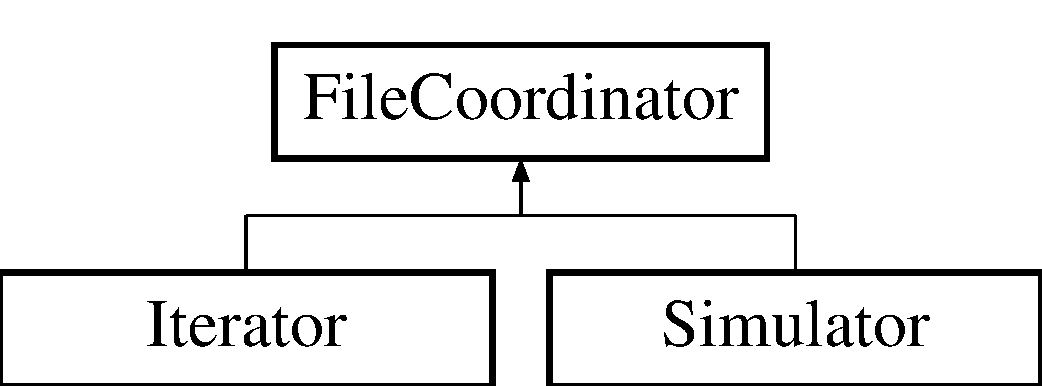
\includegraphics[height=2.000000cm]{class_file_coordinator}
\end{center}
\end{figure}
\subsubsection*{Public Types}
\begin{DoxyCompactItemize}
\item 
enum \hyperlink{class_file_coordinator_a87882b51519fff558b11f4862a021318}{file\+States} \{ \hyperlink{class_file_coordinator_a87882b51519fff558b11f4862a021318af1c825462619cd97356c2609113e828c}{R\+E\+A\+D\+\_\+\+S\+U\+C\+C\+E\+S\+S}, 
\hyperlink{class_file_coordinator_a87882b51519fff558b11f4862a021318adad0373980186384b160efe041ed22bd}{R\+E\+A\+D\+\_\+\+F\+A\+I\+L\+U\+R\+E}
 \}
\begin{DoxyCompactList}\small\item\em Specifies the states of the file being processed. \end{DoxyCompactList}\item 
enum \hyperlink{class_file_coordinator_a3675d464de774750ec143958d199891e}{save\+Types} \{ \hyperlink{class_file_coordinator_a3675d464de774750ec143958d199891ea0e8f89951a9591e7c4c9c98c79514b45}{M\+A\+T\+R\+I\+X}, 
\hyperlink{class_file_coordinator_a3675d464de774750ec143958d199891eaf405bb89eede8cfbb12aefb8c0f230b4}{E\+N\+T\+R\+O\+P\+Y}, 
\hyperlink{class_file_coordinator_a3675d464de774750ec143958d199891ea35b0a6cf33dc95857927320bfd6acce5}{W\+E\+I\+G\+H\+T\+S}, 
\hyperlink{class_file_coordinator_a3675d464de774750ec143958d199891ea25e4073fbd44c81e075066787b33a5de}{I\+T\+E\+R\+A\+T\+I\+O\+N}
 \}
\begin{DoxyCompactList}\small\item\em Specifies the types of data to be saved. \end{DoxyCompactList}\end{DoxyCompactItemize}
\subsubsection*{Public Member Functions}
\begin{DoxyCompactItemize}
\item 
string \hyperlink{class_file_coordinator_a7d382bac08ac208a283c9c41e4be6117}{get\+Full\+Path} ()
\item 
string \hyperlink{class_file_coordinator_ab15e2283157ef9c18ebbb6e9e36f9744}{get\+File\+Name} ()
\item 
string \hyperlink{class_file_coordinator_af03a39aeaffebf1f90c25591700aa046}{get\+Failure\+Message} ()
\item 
virtual \hyperlink{class_file_coordinator_a87882b51519fff558b11f4862a021318}{file\+States} \hyperlink{class_file_coordinator_a135715b1b9b4eaab42e061ebf9fd2459}{read\+File} (string file\+Name, int num\+Of\+Genes)
\end{DoxyCompactItemize}
\subsubsection*{Protected Attributes}
\begin{DoxyCompactItemize}
\item 
\hypertarget{class_file_coordinator_ab8313bec8a35d369ef65d59822dd6c68}{string \hyperlink{class_file_coordinator_ab8313bec8a35d369ef65d59822dd6c68}{F\+A\+I\+L\+U\+R\+E\+\_\+\+M\+E\+S\+S\+A\+G\+E}}\label{class_file_coordinator_ab8313bec8a35d369ef65d59822dd6c68}

\begin{DoxyCompactList}\small\item\em Failure message expressing the cause of read file failure;. \end{DoxyCompactList}\item 
\hypertarget{class_file_coordinator_aa78d3f7b41ca66e461b0ff4c8b488821}{string \hyperlink{class_file_coordinator_aa78d3f7b41ca66e461b0ff4c8b488821}{F\+O\+L\+D\+E\+R}}\label{class_file_coordinator_aa78d3f7b41ca66e461b0ff4c8b488821}

\begin{DoxyCompactList}\small\item\em Folder of the file to process;. \end{DoxyCompactList}\item 
\hypertarget{class_file_coordinator_a6d9ec231c41442f9d71ad62838bdb2fe}{string \hyperlink{class_file_coordinator_a6d9ec231c41442f9d71ad62838bdb2fe}{F\+I\+L\+E\+P\+R\+E\+F\+I\+X}}\label{class_file_coordinator_a6d9ec231c41442f9d71ad62838bdb2fe}

\begin{DoxyCompactList}\small\item\em Prefix of the file. i.\+e \char`\"{}sparse\+Transition\+\_\+\char`\"{}. \end{DoxyCompactList}\item 
\hypertarget{class_file_coordinator_ac92f75a0e19bff63fafc40217688f927}{string \hyperlink{class_file_coordinator_ac92f75a0e19bff63fafc40217688f927}{suffix}}\label{class_file_coordinator_ac92f75a0e19bff63fafc40217688f927}

\begin{DoxyCompactList}\small\item\em Suffix of the file specified by user; i.\+e \char`\"{}new\+Test\char`\"{}. \end{DoxyCompactList}\item 
\hypertarget{class_file_coordinator_a439cb1f8132fd37e04f92ac67f89c1df}{string \hyperlink{class_file_coordinator_a439cb1f8132fd37e04f92ac67f89c1df}{filename}}\label{class_file_coordinator_a439cb1f8132fd37e04f92ac67f89c1df}

\begin{DoxyCompactList}\small\item\em Name of the file; i.\+e \char`\"{}\+C\+E\+M\char`\"{}, \char`\"{}overall\char`\"{}. \end{DoxyCompactList}\item 
\hypertarget{class_file_coordinator_a73af7cec077de88eebd7a33fad13ef23}{\hyperlink{classt_matrix}{t\+Matrix} $\ast$ \hyperlink{class_file_coordinator_a73af7cec077de88eebd7a33fad13ef23}{transition}}\label{class_file_coordinator_a73af7cec077de88eebd7a33fad13ef23}

\begin{DoxyCompactList}\small\item\em The transition matrix currently being processed. \end{DoxyCompactList}\end{DoxyCompactItemize}
\subsubsection*{Private Member Functions}
\begin{DoxyCompactItemize}
\item 
virtual string \hyperlink{class_file_coordinator_a913c584fd94fdcacd120bf6f52819aad}{save\+Matrix} ()
\item 
virtual void \hyperlink{class_file_coordinator_a2d9b661099244a87012a4f7de9d3a120}{save\+Vector} (vector$<$ double $>$ \&stats, \hyperlink{class_file_coordinator_a3675d464de774750ec143958d199891e}{save\+Types} type)
\item 
virtual void \hyperlink{class_file_coordinator_a53023597e8e80b9f6bb4f7edb16b098c}{save\+Iteration} ()
\end{DoxyCompactItemize}


\subsubsection{Detailed Description}
Abstract class for file manipulations. 

This is an abstract class that declared function prototypes used for file manipulations. Classes encapsulating algorithms should subclass from this class for file interaction and should implement the virtual methods as needed. 

\subsubsection{Member Enumeration Documentation}
\hypertarget{class_file_coordinator_a87882b51519fff558b11f4862a021318}{\index{File\+Coordinator@{File\+Coordinator}!file\+States@{file\+States}}
\index{file\+States@{file\+States}!File\+Coordinator@{File\+Coordinator}}
\paragraph[{file\+States}]{\setlength{\rightskip}{0pt plus 5cm}enum {\bf File\+Coordinator\+::file\+States}}}\label{class_file_coordinator_a87882b51519fff558b11f4862a021318}


Specifies the states of the file being processed. 

The file being read could be read successfully or there might be an exception. When the state is \char`\"{}\+R\+E\+A\+D\+\_\+\+F\+A\+I\+L\+U\+R\+E\char`\"{}, a failure message will be generated for the user to correct. \begin{Desc}
\item[Enumerator]\par
\begin{description}
\index{R\+E\+A\+D\+\_\+\+S\+U\+C\+C\+E\+S\+S@{R\+E\+A\+D\+\_\+\+S\+U\+C\+C\+E\+S\+S}!File\+Coordinator@{File\+Coordinator}}\index{File\+Coordinator@{File\+Coordinator}!R\+E\+A\+D\+\_\+\+S\+U\+C\+C\+E\+S\+S@{R\+E\+A\+D\+\_\+\+S\+U\+C\+C\+E\+S\+S}}\item[{\em 
\hypertarget{class_file_coordinator_a87882b51519fff558b11f4862a021318af1c825462619cd97356c2609113e828c}{R\+E\+A\+D\+\_\+\+S\+U\+C\+C\+E\+S\+S}\label{class_file_coordinator_a87882b51519fff558b11f4862a021318af1c825462619cd97356c2609113e828c}
}]File successfully read in. \index{R\+E\+A\+D\+\_\+\+F\+A\+I\+L\+U\+R\+E@{R\+E\+A\+D\+\_\+\+F\+A\+I\+L\+U\+R\+E}!File\+Coordinator@{File\+Coordinator}}\index{File\+Coordinator@{File\+Coordinator}!R\+E\+A\+D\+\_\+\+F\+A\+I\+L\+U\+R\+E@{R\+E\+A\+D\+\_\+\+F\+A\+I\+L\+U\+R\+E}}\item[{\em 
\hypertarget{class_file_coordinator_a87882b51519fff558b11f4862a021318adad0373980186384b160efe041ed22bd}{R\+E\+A\+D\+\_\+\+F\+A\+I\+L\+U\+R\+E}\label{class_file_coordinator_a87882b51519fff558b11f4862a021318adad0373980186384b160efe041ed22bd}
}]Error occurred when reading file. \end{description}
\end{Desc}
\hypertarget{class_file_coordinator_a3675d464de774750ec143958d199891e}{\index{File\+Coordinator@{File\+Coordinator}!save\+Types@{save\+Types}}
\index{save\+Types@{save\+Types}!File\+Coordinator@{File\+Coordinator}}
\paragraph[{save\+Types}]{\setlength{\rightskip}{0pt plus 5cm}enum {\bf File\+Coordinator\+::save\+Types}}}\label{class_file_coordinator_a3675d464de774750ec143958d199891e}


Specifies the types of data to be saved. 

The types of data to be saved will be used to determine which method to be used for saving process. \begin{Desc}
\item[Enumerator]\par
\begin{description}
\index{M\+A\+T\+R\+I\+X@{M\+A\+T\+R\+I\+X}!File\+Coordinator@{File\+Coordinator}}\index{File\+Coordinator@{File\+Coordinator}!M\+A\+T\+R\+I\+X@{M\+A\+T\+R\+I\+X}}\item[{\em 
\hypertarget{class_file_coordinator_a3675d464de774750ec143958d199891ea0e8f89951a9591e7c4c9c98c79514b45}{M\+A\+T\+R\+I\+X}\label{class_file_coordinator_a3675d464de774750ec143958d199891ea0e8f89951a9591e7c4c9c98c79514b45}
}]Type M\+A\+T\+R\+I\+X is used when a transition matrix is saved;. \index{E\+N\+T\+R\+O\+P\+Y@{E\+N\+T\+R\+O\+P\+Y}!File\+Coordinator@{File\+Coordinator}}\index{File\+Coordinator@{File\+Coordinator}!E\+N\+T\+R\+O\+P\+Y@{E\+N\+T\+R\+O\+P\+Y}}\item[{\em 
\hypertarget{class_file_coordinator_a3675d464de774750ec143958d199891eaf405bb89eede8cfbb12aefb8c0f230b4}{E\+N\+T\+R\+O\+P\+Y}\label{class_file_coordinator_a3675d464de774750ec143958d199891eaf405bb89eede8cfbb12aefb8c0f230b4}
}]Type E\+N\+T\+R\+O\+P\+Y is used when saving entropies of decomposition;. \index{W\+E\+I\+G\+H\+T\+S@{W\+E\+I\+G\+H\+T\+S}!File\+Coordinator@{File\+Coordinator}}\index{File\+Coordinator@{File\+Coordinator}!W\+E\+I\+G\+H\+T\+S@{W\+E\+I\+G\+H\+T\+S}}\item[{\em 
\hypertarget{class_file_coordinator_a3675d464de774750ec143958d199891ea35b0a6cf33dc95857927320bfd6acce5}{W\+E\+I\+G\+H\+T\+S}\label{class_file_coordinator_a3675d464de774750ec143958d199891ea35b0a6cf33dc95857927320bfd6acce5}
}]Type W\+E\+I\+G\+H\+T\+S is used when saving wegits of decomposition;. \index{I\+T\+E\+R\+A\+T\+I\+O\+N@{I\+T\+E\+R\+A\+T\+I\+O\+N}!File\+Coordinator@{File\+Coordinator}}\index{File\+Coordinator@{File\+Coordinator}!I\+T\+E\+R\+A\+T\+I\+O\+N@{I\+T\+E\+R\+A\+T\+I\+O\+N}}\item[{\em 
\hypertarget{class_file_coordinator_a3675d464de774750ec143958d199891ea25e4073fbd44c81e075066787b33a5de}{I\+T\+E\+R\+A\+T\+I\+O\+N}\label{class_file_coordinator_a3675d464de774750ec143958d199891ea25e4073fbd44c81e075066787b33a5de}
}]Type I\+T\+E\+R\+A\+T\+I\+O\+N is used when saving the iteration information containing minimal entropy result. \end{description}
\end{Desc}


\subsubsection{Member Function Documentation}
\hypertarget{class_file_coordinator_af03a39aeaffebf1f90c25591700aa046}{\index{File\+Coordinator@{File\+Coordinator}!get\+Failure\+Message@{get\+Failure\+Message}}
\index{get\+Failure\+Message@{get\+Failure\+Message}!File\+Coordinator@{File\+Coordinator}}
\paragraph[{get\+Failure\+Message}]{\setlength{\rightskip}{0pt plus 5cm}string File\+Coordinator\+::get\+Failure\+Message (
\begin{DoxyParamCaption}
{}
\end{DoxyParamCaption}
)}}\label{class_file_coordinator_af03a39aeaffebf1f90c25591700aa046}
Get the failure message if exceptions happen during file manipulation process. \begin{DoxyReturn}{Returns}
The failure message. 
\end{DoxyReturn}
\hypertarget{class_file_coordinator_ab15e2283157ef9c18ebbb6e9e36f9744}{\index{File\+Coordinator@{File\+Coordinator}!get\+File\+Name@{get\+File\+Name}}
\index{get\+File\+Name@{get\+File\+Name}!File\+Coordinator@{File\+Coordinator}}
\paragraph[{get\+File\+Name}]{\setlength{\rightskip}{0pt plus 5cm}string File\+Coordinator\+::get\+File\+Name (
\begin{DoxyParamCaption}
{}
\end{DoxyParamCaption}
)}}\label{class_file_coordinator_ab15e2283157ef9c18ebbb6e9e36f9744}
Get the filename for the file that is currently being processed or created. i.\+e If full path is \char`\"{}\+Input/\+Provided/\+C\+E\+M.\+txt\char`\"{}, will return \char`\"{}\+C\+E\+M\char`\"{}. \begin{DoxyReturn}{Returns}
The name of the file(without extension) being processed. 
\end{DoxyReturn}
\hypertarget{class_file_coordinator_a7d382bac08ac208a283c9c41e4be6117}{\index{File\+Coordinator@{File\+Coordinator}!get\+Full\+Path@{get\+Full\+Path}}
\index{get\+Full\+Path@{get\+Full\+Path}!File\+Coordinator@{File\+Coordinator}}
\paragraph[{get\+Full\+Path}]{\setlength{\rightskip}{0pt plus 5cm}string File\+Coordinator\+::get\+Full\+Path (
\begin{DoxyParamCaption}
{}
\end{DoxyParamCaption}
)}}\label{class_file_coordinator_a7d382bac08ac208a283c9c41e4be6117}
Get the full path of the file that is currently being processed or created. \begin{DoxyReturn}{Returns}
The full path of the file. 
\end{DoxyReturn}
\hypertarget{class_file_coordinator_a135715b1b9b4eaab42e061ebf9fd2459}{\index{File\+Coordinator@{File\+Coordinator}!read\+File@{read\+File}}
\index{read\+File@{read\+File}!File\+Coordinator@{File\+Coordinator}}
\paragraph[{read\+File}]{\setlength{\rightskip}{0pt plus 5cm}virtual {\bf file\+States} File\+Coordinator\+::read\+File (
\begin{DoxyParamCaption}
\item[{string}]{file\+Name, }
\item[{int}]{num\+Of\+Genes}
\end{DoxyParamCaption}
)\hspace{0.3cm}{\ttfamily [virtual]}}}\label{class_file_coordinator_a135715b1b9b4eaab42e061ebf9fd2459}
A function prototype declared for reading in a transition matrix from a certain file. Overriden by \char`\"{}\+Iterator\char`\"{} class. 
\begin{DoxyParams}{Parameters}
{\em file\+Name} & The name of the file, without extension and path; \\
\hline
{\em num\+Of\+Genes} & The number of genes corresponding to the matrix in the file; \\
\hline
\end{DoxyParams}
\begin{DoxyReturn}{Returns}
A file\+States indicating whether the reading process is successful. 
\end{DoxyReturn}


Reimplemented in \hyperlink{class_iterator_a3da499aae907e1d3c1e98d41d986718b}{Iterator}.

\hypertarget{class_file_coordinator_a53023597e8e80b9f6bb4f7edb16b098c}{\index{File\+Coordinator@{File\+Coordinator}!save\+Iteration@{save\+Iteration}}
\index{save\+Iteration@{save\+Iteration}!File\+Coordinator@{File\+Coordinator}}
\paragraph[{save\+Iteration}]{\setlength{\rightskip}{0pt plus 5cm}virtual void File\+Coordinator\+::save\+Iteration (
\begin{DoxyParamCaption}
{}
\end{DoxyParamCaption}
)\hspace{0.3cm}{\ttfamily [private]}, {\ttfamily [virtual]}}}\label{class_file_coordinator_a53023597e8e80b9f6bb4f7edb16b098c}
Saves iteration information into current file. 

Reimplemented in \hyperlink{class_iterator_a2bd1f005ae0c283af59e9b5698934d88}{Iterator}.

\hypertarget{class_file_coordinator_a913c584fd94fdcacd120bf6f52819aad}{\index{File\+Coordinator@{File\+Coordinator}!save\+Matrix@{save\+Matrix}}
\index{save\+Matrix@{save\+Matrix}!File\+Coordinator@{File\+Coordinator}}
\paragraph[{save\+Matrix}]{\setlength{\rightskip}{0pt plus 5cm}virtual string File\+Coordinator\+::save\+Matrix (
\begin{DoxyParamCaption}
{}
\end{DoxyParamCaption}
)\hspace{0.3cm}{\ttfamily [private]}, {\ttfamily [virtual]}}}\label{class_file_coordinator_a913c584fd94fdcacd120bf6f52819aad}
Saves the transition matrix to current file. \begin{DoxyReturn}{Returns}
Returns the full path of the file. 
\end{DoxyReturn}


Reimplemented in \hyperlink{class_simulator_a1270d2e2eeaa4aa3284e2d74a8644bc3}{Simulator}.

\hypertarget{class_file_coordinator_a2d9b661099244a87012a4f7de9d3a120}{\index{File\+Coordinator@{File\+Coordinator}!save\+Vector@{save\+Vector}}
\index{save\+Vector@{save\+Vector}!File\+Coordinator@{File\+Coordinator}}
\paragraph[{save\+Vector}]{\setlength{\rightskip}{0pt plus 5cm}virtual void File\+Coordinator\+::save\+Vector (
\begin{DoxyParamCaption}
\item[{vector$<$ double $>$ \&}]{stats, }
\item[{{\bf save\+Types}}]{type}
\end{DoxyParamCaption}
)\hspace{0.3cm}{\ttfamily [private]}, {\ttfamily [virtual]}}}\label{class_file_coordinator_a2d9b661099244a87012a4f7de9d3a120}
Saves a vector into the current file, depending on the parameters. 
\begin{DoxyParams}{Parameters}
{\em stats} & The vector data to save. \\
\hline
{\em type} & The save\+Type specifying the type of data. i.\+e E\+N\+T\+R\+O\+P\+Y, W\+E\+I\+G\+H\+T\+S \\
\hline
\end{DoxyParams}


Reimplemented in \hyperlink{class_iterator_a17d24545df8bc3245ef4d31928a85186}{Iterator}.



The documentation for this class was generated from the following file\+:\begin{DoxyCompactItemize}
\item 
\hyperlink{_file_coordinator_8h}{File\+Coordinator.\+h}\end{DoxyCompactItemize}

\hypertarget{class_interactor}{\subsection{Interactor Class Reference}
\label{class_interactor}\index{Interactor@{Interactor}}
}


An abstract controller class that contains method prototypes or basic implementations of methods for further overriding.  




{\ttfamily \#include $<$Interactor.\+h$>$}

Inheritance diagram for Interactor\+:\begin{figure}[H]
\begin{center}
\leavevmode
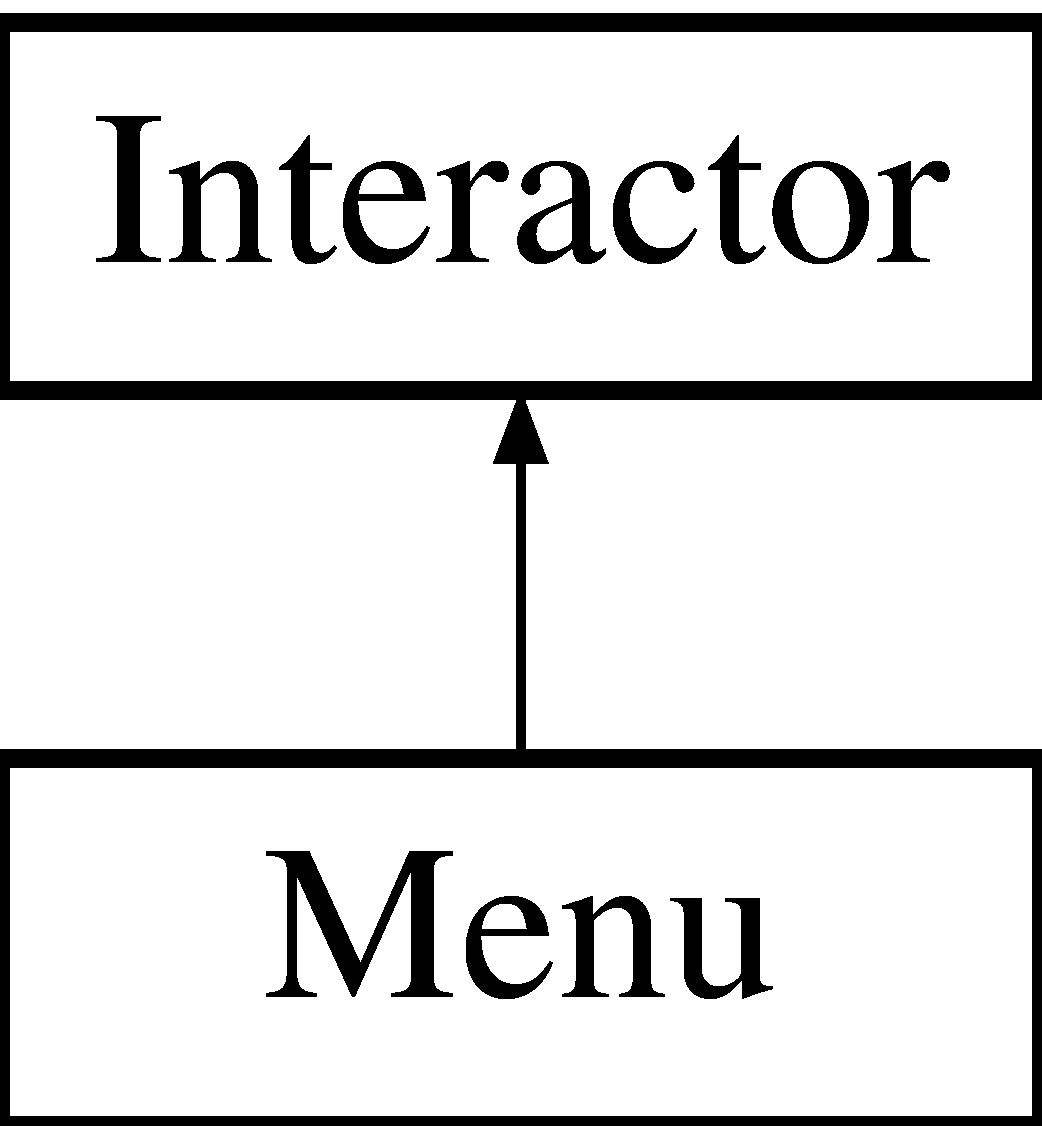
\includegraphics[height=2.000000cm]{class_interactor}
\end{center}
\end{figure}
\subsubsection*{Protected Member Functions}
\begin{DoxyCompactItemize}
\item 
void \hyperlink{class_interactor_ab67e4ff9ff5d44ee2001e7700dfeb164}{initialize\+Iterator} ()
\item 
void \hyperlink{class_interactor_a8416bb98d11e11b841db245e93c98853}{initialize\+Simulator} ()
\item 
void \hyperlink{class_interactor_aeb10be4d589b66a8624d7221f7600f87}{initialize\+Iterator} (string suffix, string file\+Name, int num\+Of\+Genes)
\item 
void \hyperlink{class_interactor_a1a9260b3dbc1c1f87933f98fadedb979}{initialize\+Simulator} (int num\+Of\+Genes, int simulate\+Type, string suffix)
\item 
string \hyperlink{class_interactor_a20edc6190516131bec1f697b81410550}{start\+Iterator} ()
\item 
string \hyperlink{class_interactor_a60a3be74e1e954f23182fab7b638164e}{start\+Simulator} ()
\end{DoxyCompactItemize}
\subsubsection*{Private Member Functions}
\begin{DoxyCompactItemize}
\item 
virtual void \hyperlink{class_interactor_a63d581b5afbf258b25915b318c1216c7}{get\+Simulator\+Params} (int \&num\+Of\+Genes, int \&simulate\+Type, string \&suffix)=0
\item 
virtual bool \hyperlink{class_interactor_a6e98daf626d09b585375eec2d5311f25}{get\+Iterator\+Params} (\hyperlink{class_iterator_a1eb24c519953c2a333ea4a345b0c679c}{Iterator\+::\+Iterator\+Status} \&status, \hyperlink{class_iterator_a68bc1c5e7ad39ed78690beaa8a607430}{Iterator\+::\+Random\+Types} \&type, string \&file\+Name, string \&suffix, int \&num\+Of\+Genes)=0
\item 
virtual string \hyperlink{class_interactor_af3d8accfc60634bf82be9c438c0b9400}{get\+Suffix} ()=0
\item 
virtual void \hyperlink{class_interactor_ac2282b0725d5bd6216edb0f2ea4dd421}{test\+All\+On\+Simulator} ()=0
\item 
virtual void \hyperlink{class_interactor_aeeec69df23673e87530a1b1db98998ee}{test\+All\+On\+Iterator} (\hyperlink{class_iterator_a1eb24c519953c2a333ea4a345b0c679c}{Iterator\+::\+Iterator\+Status} status)=0
\end{DoxyCompactItemize}


\subsubsection{Detailed Description}
An abstract controller class that contains method prototypes or basic implementations of methods for further overriding. 

\subsubsection{Member Function Documentation}
\hypertarget{class_interactor_a6e98daf626d09b585375eec2d5311f25}{\index{Interactor@{Interactor}!get\+Iterator\+Params@{get\+Iterator\+Params}}
\index{get\+Iterator\+Params@{get\+Iterator\+Params}!Interactor@{Interactor}}
\paragraph[{get\+Iterator\+Params}]{\setlength{\rightskip}{0pt plus 5cm}virtual bool Interactor\+::get\+Iterator\+Params (
\begin{DoxyParamCaption}
\item[{{\bf Iterator\+::\+Iterator\+Status} \&}]{status, }
\item[{{\bf Iterator\+::\+Random\+Types} \&}]{type, }
\item[{string \&}]{file\+Name, }
\item[{string \&}]{suffix, }
\item[{int \&}]{num\+Of\+Genes}
\end{DoxyParamCaption}
)\hspace{0.3cm}{\ttfamily [private]}, {\ttfamily [pure virtual]}}}\label{class_interactor_a6e98daf626d09b585375eec2d5311f25}
Function prototype for getting \hyperlink{class_iterator}{Iterator} parameters. 
\begin{DoxyParams}{Parameters}
{\em status} & \hyperlink{class_iterator}{Iterator} status, S\+I\+M\+U\+L\+A\+T\+E\+D or P\+R\+O\+V\+I\+D\+E\+D. \\
\hline
\end{DoxyParams}
\begin{DoxySeeAlso}{See Also}
\hyperlink{class_iterator_a1eb24c519953c2a333ea4a345b0c679c}{Iterator\+::\+Iterator\+Status} 
\end{DoxySeeAlso}

\begin{DoxyParams}{Parameters}
{\em type} & Iteration type. \\
\hline
\end{DoxyParams}
\begin{DoxySeeAlso}{See Also}
\hyperlink{class_iterator_a68bc1c5e7ad39ed78690beaa8a607430}{Iterator\+::\+Random\+Types} 
\end{DoxySeeAlso}

\begin{DoxyParams}{Parameters}
{\em file\+Name} & The input filename. i.\+e \char`\"{}overall\char`\"{} for \char`\"{}overall.\+txt\char`\"{} \\
\hline
{\em suffix} & File suffix added to output file \\
\hline
{\em num\+Of\+Genes} & Number of genes corresponding to the input file \\
\hline
\end{DoxyParams}
\begin{DoxyReturn}{Returns}
True if the \hyperlink{class_iterator}{Iterator} parameters are default values 
\end{DoxyReturn}


Implemented in \hyperlink{class_menu_ac759d0525a0736f421e8dfd443b1177c}{Menu}.

\hypertarget{class_interactor_a63d581b5afbf258b25915b318c1216c7}{\index{Interactor@{Interactor}!get\+Simulator\+Params@{get\+Simulator\+Params}}
\index{get\+Simulator\+Params@{get\+Simulator\+Params}!Interactor@{Interactor}}
\paragraph[{get\+Simulator\+Params}]{\setlength{\rightskip}{0pt plus 5cm}virtual void Interactor\+::get\+Simulator\+Params (
\begin{DoxyParamCaption}
\item[{int \&}]{num\+Of\+Genes, }
\item[{int \&}]{simulate\+Type, }
\item[{string \&}]{suffix}
\end{DoxyParamCaption}
)\hspace{0.3cm}{\ttfamily [private]}, {\ttfamily [pure virtual]}}}\label{class_interactor_a63d581b5afbf258b25915b318c1216c7}
Function prototype for getting \hyperlink{class_simulator}{Simulator} parameters. 
\begin{DoxyParams}{Parameters}
{\em num\+Of\+Genes} & Number of genes to simulate \\
\hline
{\em simulate\+Type} & Type of simulation, default is S\+P\+A\+R\+S\+E \\
\hline
{\em suffix} & Suffix added to the end of output file \\
\hline
\end{DoxyParams}


Implemented in \hyperlink{class_menu_a893fd3c7d9e4bc5e32d4e2e20d8da804}{Menu}.

\hypertarget{class_interactor_af3d8accfc60634bf82be9c438c0b9400}{\index{Interactor@{Interactor}!get\+Suffix@{get\+Suffix}}
\index{get\+Suffix@{get\+Suffix}!Interactor@{Interactor}}
\paragraph[{get\+Suffix}]{\setlength{\rightskip}{0pt plus 5cm}virtual string Interactor\+::get\+Suffix (
\begin{DoxyParamCaption}
{}
\end{DoxyParamCaption}
)\hspace{0.3cm}{\ttfamily [private]}, {\ttfamily [pure virtual]}}}\label{class_interactor_af3d8accfc60634bf82be9c438c0b9400}
Prototype for the method used to get file suffix from user \begin{DoxyReturn}{Returns}
The file suffix provided by the user 
\end{DoxyReturn}


Implemented in \hyperlink{class_menu_ab5b08e13a2db9ae41ac9e9696473a143}{Menu}.

\hypertarget{class_interactor_ab67e4ff9ff5d44ee2001e7700dfeb164}{\index{Interactor@{Interactor}!initialize\+Iterator@{initialize\+Iterator}}
\index{initialize\+Iterator@{initialize\+Iterator}!Interactor@{Interactor}}
\paragraph[{initialize\+Iterator}]{\setlength{\rightskip}{0pt plus 5cm}void Interactor\+::initialize\+Iterator (
\begin{DoxyParamCaption}
{}
\end{DoxyParamCaption}
)\hspace{0.3cm}{\ttfamily [protected]}}}\label{class_interactor_ab67e4ff9ff5d44ee2001e7700dfeb164}
Initialize the owned \hyperlink{class_iterator}{Iterator} object. \hypertarget{class_interactor_aeb10be4d589b66a8624d7221f7600f87}{\index{Interactor@{Interactor}!initialize\+Iterator@{initialize\+Iterator}}
\index{initialize\+Iterator@{initialize\+Iterator}!Interactor@{Interactor}}
\paragraph[{initialize\+Iterator}]{\setlength{\rightskip}{0pt plus 5cm}void Interactor\+::initialize\+Iterator (
\begin{DoxyParamCaption}
\item[{string}]{suffix, }
\item[{string}]{file\+Name, }
\item[{int}]{num\+Of\+Genes}
\end{DoxyParamCaption}
)\hspace{0.3cm}{\ttfamily [protected]}}}\label{class_interactor_aeb10be4d589b66a8624d7221f7600f87}
Overloaded version, initialize the \hyperlink{class_iterator}{Iterator} with specified params. 
\begin{DoxyParams}{Parameters}
{\em suffix} & File suffix added to the end of the file \\
\hline
{\em file\+Name} & The file name of input \\
\hline
{\em num\+Of\+Genes} & Number of genes corresponding to the input file\\
\hline
\end{DoxyParams}
\begin{DoxyNote}{Note}
This method is called by the \hyperlink{class_interactor_ab67e4ff9ff5d44ee2001e7700dfeb164}{Interactor\+::initialize\+Iterator()} method internally. 
\end{DoxyNote}
\hypertarget{class_interactor_a8416bb98d11e11b841db245e93c98853}{\index{Interactor@{Interactor}!initialize\+Simulator@{initialize\+Simulator}}
\index{initialize\+Simulator@{initialize\+Simulator}!Interactor@{Interactor}}
\paragraph[{initialize\+Simulator}]{\setlength{\rightskip}{0pt plus 5cm}void Interactor\+::initialize\+Simulator (
\begin{DoxyParamCaption}
{}
\end{DoxyParamCaption}
)\hspace{0.3cm}{\ttfamily [protected]}}}\label{class_interactor_a8416bb98d11e11b841db245e93c98853}
Initialize the owned \hyperlink{class_simulator}{Simulator} object. \hypertarget{class_interactor_a1a9260b3dbc1c1f87933f98fadedb979}{\index{Interactor@{Interactor}!initialize\+Simulator@{initialize\+Simulator}}
\index{initialize\+Simulator@{initialize\+Simulator}!Interactor@{Interactor}}
\paragraph[{initialize\+Simulator}]{\setlength{\rightskip}{0pt plus 5cm}void Interactor\+::initialize\+Simulator (
\begin{DoxyParamCaption}
\item[{int}]{num\+Of\+Genes, }
\item[{int}]{simulate\+Type, }
\item[{string}]{suffix}
\end{DoxyParamCaption}
)\hspace{0.3cm}{\ttfamily [protected]}}}\label{class_interactor_a1a9260b3dbc1c1f87933f98fadedb979}
Overloaded version, initialize the \hyperlink{class_simulator}{Simulator} with specified params. 
\begin{DoxyParams}{Parameters}
{\em num\+Of\+Genes} & Number of genes the user wants to simulate \\
\hline
{\em simulate\+Type} & The type of simulation, the default is S\+P\+A\+R\+S\+E \\
\hline
{\em suffix} & The file suffix of the output file\\
\hline
\end{DoxyParams}
\begin{DoxyNote}{Note}
This method is called by the \hyperlink{class_interactor_a8416bb98d11e11b841db245e93c98853}{Interactor\+::initialize\+Simulator()} method internally. 
\end{DoxyNote}
\hypertarget{class_interactor_a20edc6190516131bec1f697b81410550}{\index{Interactor@{Interactor}!start\+Iterator@{start\+Iterator}}
\index{start\+Iterator@{start\+Iterator}!Interactor@{Interactor}}
\paragraph[{start\+Iterator}]{\setlength{\rightskip}{0pt plus 5cm}string Interactor\+::start\+Iterator (
\begin{DoxyParamCaption}
{}
\end{DoxyParamCaption}
)\hspace{0.3cm}{\ttfamily [protected]}}}\label{class_interactor_a20edc6190516131bec1f697b81410550}
Starts the \hyperlink{class_iterator}{Iterator} object, will be overridden in concrete implementation. \begin{DoxyReturn}{Returns}
A message indicating the status of the \hyperlink{class_iterator}{Iterator} 
\end{DoxyReturn}
\hypertarget{class_interactor_a60a3be74e1e954f23182fab7b638164e}{\index{Interactor@{Interactor}!start\+Simulator@{start\+Simulator}}
\index{start\+Simulator@{start\+Simulator}!Interactor@{Interactor}}
\paragraph[{start\+Simulator}]{\setlength{\rightskip}{0pt plus 5cm}string Interactor\+::start\+Simulator (
\begin{DoxyParamCaption}
{}
\end{DoxyParamCaption}
)\hspace{0.3cm}{\ttfamily [protected]}}}\label{class_interactor_a60a3be74e1e954f23182fab7b638164e}
Starts the \hyperlink{class_simulator}{Simulator} object, will be overridden in concrete implementation. \begin{DoxyReturn}{Returns}
A message indicating the status of the \hyperlink{class_simulator}{Simulator} 
\end{DoxyReturn}
\hypertarget{class_interactor_aeeec69df23673e87530a1b1db98998ee}{\index{Interactor@{Interactor}!test\+All\+On\+Iterator@{test\+All\+On\+Iterator}}
\index{test\+All\+On\+Iterator@{test\+All\+On\+Iterator}!Interactor@{Interactor}}
\paragraph[{test\+All\+On\+Iterator}]{\setlength{\rightskip}{0pt plus 5cm}virtual void Interactor\+::test\+All\+On\+Iterator (
\begin{DoxyParamCaption}
\item[{{\bf Iterator\+::\+Iterator\+Status}}]{status}
\end{DoxyParamCaption}
)\hspace{0.3cm}{\ttfamily [private]}, {\ttfamily [pure virtual]}}}\label{class_interactor_aeeec69df23673e87530a1b1db98998ee}
Test all prepared iteration cases, either P\+R\+O\+V\+I\+D\+E\+D or S\+I\+M\+U\+L\+A\+T\+E\+D 
\begin{DoxyParams}{Parameters}
{\em status} & Input file type. P\+R\+O\+V\+I\+D\+E\+D or S\+I\+M\+U\+L\+A\+T\+E\+D. \\
\hline
\end{DoxyParams}


Implemented in \hyperlink{class_menu_a4ff4dfbd63a558ed2a6aa79fbde05eba}{Menu}.

\hypertarget{class_interactor_ac2282b0725d5bd6216edb0f2ea4dd421}{\index{Interactor@{Interactor}!test\+All\+On\+Simulator@{test\+All\+On\+Simulator}}
\index{test\+All\+On\+Simulator@{test\+All\+On\+Simulator}!Interactor@{Interactor}}
\paragraph[{test\+All\+On\+Simulator}]{\setlength{\rightskip}{0pt plus 5cm}virtual void Interactor\+::test\+All\+On\+Simulator (
\begin{DoxyParamCaption}
{}
\end{DoxyParamCaption}
)\hspace{0.3cm}{\ttfamily [private]}, {\ttfamily [pure virtual]}}}\label{class_interactor_ac2282b0725d5bd6216edb0f2ea4dd421}
Test all prepared simulation cases. 

Implemented in \hyperlink{class_menu_a27538c5e2650251e98ed91257b0a2ba8}{Menu}.



The documentation for this class was generated from the following files\+:\begin{DoxyCompactItemize}
\item 
\hyperlink{_interactor_8h}{Interactor.\+h}\item 
Interactor.\+cpp\end{DoxyCompactItemize}

\hypertarget{class_iterator}{\subsection{Iterator Class Reference}
\label{class_iterator}\index{Iterator@{Iterator}}
}


This class encapsulates the functionality of an inverse iterator.  




{\ttfamily \#include $<$Iterator.\+h$>$}

Inheritance diagram for Iterator\+:\begin{figure}[H]
\begin{center}
\leavevmode
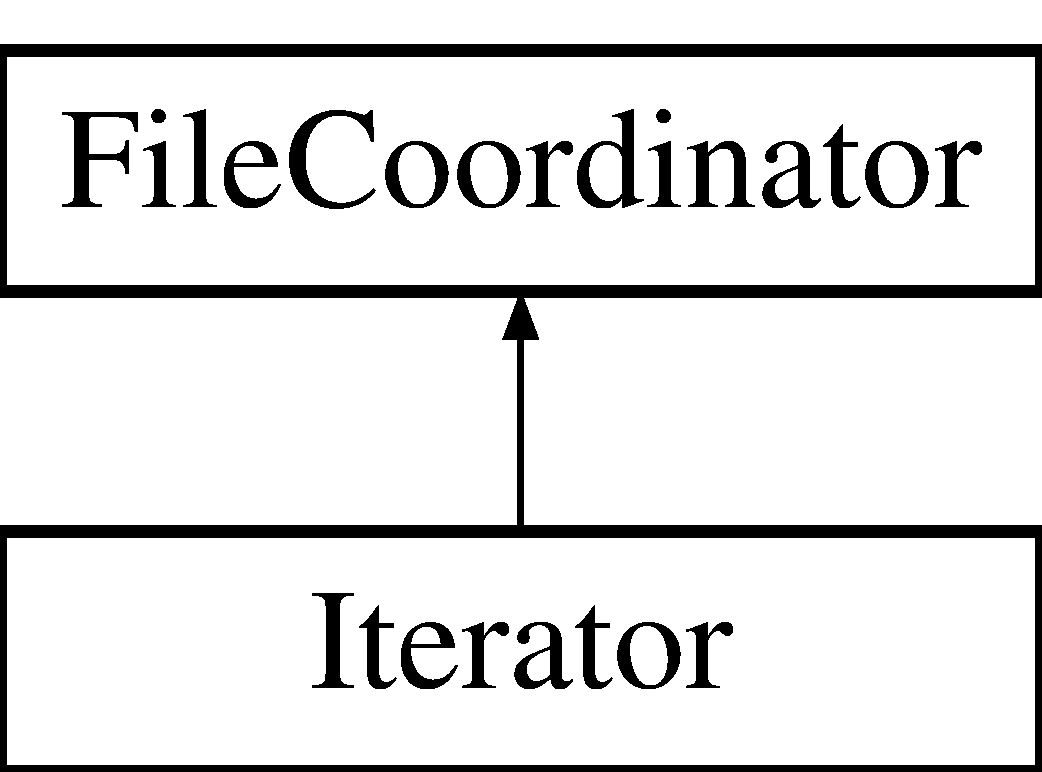
\includegraphics[height=2.000000cm]{class_iterator}
\end{center}
\end{figure}
\subsubsection*{Public Types}
\begin{DoxyCompactItemize}
\item 
enum \hyperlink{class_iterator_a1eb24c519953c2a333ea4a345b0c679c}{Iterator\+Status} \{ \hyperlink{class_iterator_a1eb24c519953c2a333ea4a345b0c679ca4628ad7429670e1077771e61b8bf62e8}{S\+I\+M\+U\+L\+A\+T\+E\+D}, 
\hyperlink{class_iterator_a1eb24c519953c2a333ea4a345b0c679ca5988fd5ab1694c99fea267cb1bd5b980}{P\+R\+O\+V\+I\+D\+E\+D}, 
\hyperlink{class_iterator_a1eb24c519953c2a333ea4a345b0c679ca47bbd9862188e6e2599aeb2396c39465}{E\+R\+R\+O\+R}, 
\hyperlink{class_iterator_a1eb24c519953c2a333ea4a345b0c679caf2fc3a710537acfd818d4b982779176e}{R\+E\+A\+D\+Y}
 \}
\begin{DoxyCompactList}\small\item\em The status of the \hyperlink{class_iterator}{Iterator}, what kind of input file it is dealing with. \end{DoxyCompactList}\item 
enum \hyperlink{class_iterator_a68bc1c5e7ad39ed78690beaa8a607430}{Random\+Types} \{ \\*
\hyperlink{class_iterator_a68bc1c5e7ad39ed78690beaa8a607430a1376e2aba7a2d8ff9240ed369a5bc08b}{Q\+U\+A\+D\+R\+A\+T\+I\+C}, 
\hyperlink{class_iterator_a68bc1c5e7ad39ed78690beaa8a607430a44ed6f57f51bfc11730908f722fdbb5f}{U\+N\+I\+F\+O\+R\+M}, 
\hyperlink{class_iterator_a68bc1c5e7ad39ed78690beaa8a607430aad4185989c35b8c829dcafe0522ac05d}{C\+U\+B\+I\+C}, 
\hyperlink{class_iterator_a68bc1c5e7ad39ed78690beaa8a607430a0df1706a866c50be36b9fe29db81af26}{M\+A\+X\+I\+M\+U\+M}, 
\\*
\hyperlink{class_iterator_a68bc1c5e7ad39ed78690beaa8a607430ac26704076bf61ec7a63ef3ece6440a05}{O\+P\+T\+I\+M\+A\+L}, 
\hyperlink{class_iterator_a68bc1c5e7ad39ed78690beaa8a607430a6a17018cada1b3e646688ff845888f8d}{D\+E\+F\+A\+U\+L\+T}
 \}
\begin{DoxyCompactList}\small\item\em The algorithms used to conduct the inverse iteration. \end{DoxyCompactList}\end{DoxyCompactItemize}
\subsubsection*{Public Member Functions}
\begin{DoxyCompactItemize}
\item 
\hyperlink{class_iterator_ab920b49c3035b9ca62557f9c211a9a12}{Iterator} (\hyperlink{class_iterator_a1eb24c519953c2a333ea4a345b0c679c}{Iterator\+Status} status=\hyperlink{class_iterator_a1eb24c519953c2a333ea4a345b0c679ca5988fd5ab1694c99fea267cb1bd5b980}{P\+R\+O\+V\+I\+D\+E\+D}, \hyperlink{class_iterator_a68bc1c5e7ad39ed78690beaa8a607430}{Random\+Types} types=\hyperlink{class_iterator_a68bc1c5e7ad39ed78690beaa8a607430ac26704076bf61ec7a63ef3ece6440a05}{O\+P\+T\+I\+M\+A\+L})
\item 
void \hyperlink{class_iterator_a39dd825e64aad150068b7b482685f264}{iterate} ()
\item 
bool \hyperlink{class_iterator_aff62fb96b13fa2d1d9ec489d413f7f54}{sanity\+Check} ()
\item 
virtual \hyperlink{class_file_coordinator_a87882b51519fff558b11f4862a021318}{file\+States} \hyperlink{class_iterator_a3da499aae907e1d3c1e98d41d986718b}{read\+File} (string file\+Name, int num\+Of\+Genes)
\end{DoxyCompactItemize}
\subsubsection*{Static Public Attributes}
\begin{DoxyCompactItemize}
\item 
static vector$<$ string $>$ \hyperlink{class_iterator_ad223ae399ddcff5d47b4991cf981932c}{R\+A\+N\+D\+O\+M\+\_\+\+T\+Y\+P\+E}
\end{DoxyCompactItemize}
\subsubsection*{Private Member Functions}
\begin{DoxyCompactItemize}
\item 
double \hyperlink{class_iterator_ac6937ada533622f876cabb537a1718c3}{iterate\+Once} ()
\item 
double \hyperlink{class_iterator_a2f3034192d0795b138b623a9101be1d0}{deterministic\+Iterate} ()
\item 
double \hyperlink{class_iterator_a1706477265276cdc503b99be64e63c12}{calculate\+Entropy} (vector$<$ double $>$ \&input\+Weights)
\item 
int \hyperlink{class_iterator_a94446a4d14889f3e9f354775916fd9b9}{choose\+Entry} (map$<$ int, double $>$ \&column, \hyperlink{class_iterator_a68bc1c5e7ad39ed78690beaa8a607430}{Random\+Types} type=\hyperlink{class_iterator_a68bc1c5e7ad39ed78690beaa8a607430a1376e2aba7a2d8ff9240ed369a5bc08b}{Q\+U\+A\+D\+R\+A\+T\+I\+C})
\item 
virtual void \hyperlink{class_iterator_a17d24545df8bc3245ef4d31928a85186}{save\+Vector} (vector$<$ double $>$ \&stats, \hyperlink{class_file_coordinator_a3675d464de774750ec143958d199891e}{save\+Types} type)
\item 
virtual void \hyperlink{class_iterator_a2bd1f005ae0c283af59e9b5698934d88}{save\+Iteration} ()
\end{DoxyCompactItemize}
\subsubsection*{Additional Inherited Members}


\subsubsection{Detailed Description}
This class encapsulates the functionality of an inverse iterator. 

The \hyperlink{class_iterator}{Iterator} inherits from \hyperlink{class_file_coordinator}{File\+Coordinator} to use the file-\/related manipulations. The methods used for iteration are separated into two categories \+: Random and Deterministic. The currently used \char`\"{}\+Optimal\char`\"{} algorithm is a deterministic algorithm. The algorithm and input file type for iteration could be set when initializing the object, like \+:


\begin{DoxyCode}
\hyperlink{class_iterator}{Iterator}* myIterator = \textcolor{keyword}{new} \hyperlink{class_iterator_ab920b49c3035b9ca62557f9c211a9a12}{Iterator}(IteratorStatus::PROVIDED, RandomTypes::OPTIMAL);
\end{DoxyCode}
 It can also be set later by invoking the \char`\"{}set\+Type\char`\"{} method, like\+:


\begin{DoxyCode}
myIterator->setType(RandomTypes::MAXIMUM);
myIterator->setIteratorStatus(IteratorStatus::SIMULATED);
\end{DoxyCode}


To let the \hyperlink{class_iterator}{Iterator} object work, clients only need to call the public method \char`\"{}iterate\char`\"{} after configuration.


\begin{DoxyCode}
myIterator->\hyperlink{class_iterator_a39dd825e64aad150068b7b482685f264}{iterate}();
\end{DoxyCode}
 

\subsubsection{Member Enumeration Documentation}
\hypertarget{class_iterator_a1eb24c519953c2a333ea4a345b0c679c}{\index{Iterator@{Iterator}!Iterator\+Status@{Iterator\+Status}}
\index{Iterator\+Status@{Iterator\+Status}!Iterator@{Iterator}}
\paragraph[{Iterator\+Status}]{\setlength{\rightskip}{0pt plus 5cm}enum {\bf Iterator\+::\+Iterator\+Status}}}\label{class_iterator_a1eb24c519953c2a333ea4a345b0c679c}


The status of the \hyperlink{class_iterator}{Iterator}, what kind of input file it is dealing with. 

\begin{Desc}
\item[Enumerator]\par
\begin{description}
\index{S\+I\+M\+U\+L\+A\+T\+E\+D@{S\+I\+M\+U\+L\+A\+T\+E\+D}!Iterator@{Iterator}}\index{Iterator@{Iterator}!S\+I\+M\+U\+L\+A\+T\+E\+D@{S\+I\+M\+U\+L\+A\+T\+E\+D}}\item[{\em 
\hypertarget{class_iterator_a1eb24c519953c2a333ea4a345b0c679ca4628ad7429670e1077771e61b8bf62e8}{S\+I\+M\+U\+L\+A\+T\+E\+D}\label{class_iterator_a1eb24c519953c2a333ea4a345b0c679ca4628ad7429670e1077771e61b8bf62e8}
}]\hyperlink{class_iterator}{Iterator} will iterate on S\+I\+M\+U\+L\+A\+T\+E\+D data. \index{P\+R\+O\+V\+I\+D\+E\+D@{P\+R\+O\+V\+I\+D\+E\+D}!Iterator@{Iterator}}\index{Iterator@{Iterator}!P\+R\+O\+V\+I\+D\+E\+D@{P\+R\+O\+V\+I\+D\+E\+D}}\item[{\em 
\hypertarget{class_iterator_a1eb24c519953c2a333ea4a345b0c679ca5988fd5ab1694c99fea267cb1bd5b980}{P\+R\+O\+V\+I\+D\+E\+D}\label{class_iterator_a1eb24c519953c2a333ea4a345b0c679ca5988fd5ab1694c99fea267cb1bd5b980}
}]\hyperlink{class_iterator}{Iterator} will iterate on P\+R\+O\+V\+I\+D\+E\+D real data. \index{E\+R\+R\+O\+R@{E\+R\+R\+O\+R}!Iterator@{Iterator}}\index{Iterator@{Iterator}!E\+R\+R\+O\+R@{E\+R\+R\+O\+R}}\item[{\em 
\hypertarget{class_iterator_a1eb24c519953c2a333ea4a345b0c679ca47bbd9862188e6e2599aeb2396c39465}{E\+R\+R\+O\+R}\label{class_iterator_a1eb24c519953c2a333ea4a345b0c679ca47bbd9862188e6e2599aeb2396c39465}
}]\hyperlink{class_iterator}{Iterator} is in error status. \index{R\+E\+A\+D\+Y@{R\+E\+A\+D\+Y}!Iterator@{Iterator}}\index{Iterator@{Iterator}!R\+E\+A\+D\+Y@{R\+E\+A\+D\+Y}}\item[{\em 
\hypertarget{class_iterator_a1eb24c519953c2a333ea4a345b0c679caf2fc3a710537acfd818d4b982779176e}{R\+E\+A\+D\+Y}\label{class_iterator_a1eb24c519953c2a333ea4a345b0c679caf2fc3a710537acfd818d4b982779176e}
}]\hyperlink{class_iterator}{Iterator} is ready to start working. \end{description}
\end{Desc}
\hypertarget{class_iterator_a68bc1c5e7ad39ed78690beaa8a607430}{\index{Iterator@{Iterator}!Random\+Types@{Random\+Types}}
\index{Random\+Types@{Random\+Types}!Iterator@{Iterator}}
\paragraph[{Random\+Types}]{\setlength{\rightskip}{0pt plus 5cm}enum {\bf Iterator\+::\+Random\+Types}}}\label{class_iterator_a68bc1c5e7ad39ed78690beaa8a607430}


The algorithms used to conduct the inverse iteration. 

Although called \char`\"{}\+Random\+Types\char`\"{}, this enumeration actually contains both random and deterministic algorithms. Moreover, clients can add self-\/developed algorithms into the enumeration. \begin{Desc}
\item[Enumerator]\par
\begin{description}
\index{Q\+U\+A\+D\+R\+A\+T\+I\+C@{Q\+U\+A\+D\+R\+A\+T\+I\+C}!Iterator@{Iterator}}\index{Iterator@{Iterator}!Q\+U\+A\+D\+R\+A\+T\+I\+C@{Q\+U\+A\+D\+R\+A\+T\+I\+C}}\item[{\em 
\hypertarget{class_iterator_a68bc1c5e7ad39ed78690beaa8a607430a1376e2aba7a2d8ff9240ed369a5bc08b}{Q\+U\+A\+D\+R\+A\+T\+I\+C}\label{class_iterator_a68bc1c5e7ad39ed78690beaa8a607430a1376e2aba7a2d8ff9240ed369a5bc08b}
}]A random algorithm, refer to the report for details. \index{U\+N\+I\+F\+O\+R\+M@{U\+N\+I\+F\+O\+R\+M}!Iterator@{Iterator}}\index{Iterator@{Iterator}!U\+N\+I\+F\+O\+R\+M@{U\+N\+I\+F\+O\+R\+M}}\item[{\em 
\hypertarget{class_iterator_a68bc1c5e7ad39ed78690beaa8a607430a44ed6f57f51bfc11730908f722fdbb5f}{U\+N\+I\+F\+O\+R\+M}\label{class_iterator_a68bc1c5e7ad39ed78690beaa8a607430a44ed6f57f51bfc11730908f722fdbb5f}
}]A random algorithm, refer to the report for details. \index{C\+U\+B\+I\+C@{C\+U\+B\+I\+C}!Iterator@{Iterator}}\index{Iterator@{Iterator}!C\+U\+B\+I\+C@{C\+U\+B\+I\+C}}\item[{\em 
\hypertarget{class_iterator_a68bc1c5e7ad39ed78690beaa8a607430aad4185989c35b8c829dcafe0522ac05d}{C\+U\+B\+I\+C}\label{class_iterator_a68bc1c5e7ad39ed78690beaa8a607430aad4185989c35b8c829dcafe0522ac05d}
}]A random algorithm, refer to the report for details. \index{M\+A\+X\+I\+M\+U\+M@{M\+A\+X\+I\+M\+U\+M}!Iterator@{Iterator}}\index{Iterator@{Iterator}!M\+A\+X\+I\+M\+U\+M@{M\+A\+X\+I\+M\+U\+M}}\item[{\em 
\hypertarget{class_iterator_a68bc1c5e7ad39ed78690beaa8a607430a0df1706a866c50be36b9fe29db81af26}{M\+A\+X\+I\+M\+U\+M}\label{class_iterator_a68bc1c5e7ad39ed78690beaa8a607430a0df1706a866c50be36b9fe29db81af26}
}]Deterministic algorithm, refer to the report for details. \index{O\+P\+T\+I\+M\+A\+L@{O\+P\+T\+I\+M\+A\+L}!Iterator@{Iterator}}\index{Iterator@{Iterator}!O\+P\+T\+I\+M\+A\+L@{O\+P\+T\+I\+M\+A\+L}}\item[{\em 
\hypertarget{class_iterator_a68bc1c5e7ad39ed78690beaa8a607430ac26704076bf61ec7a63ef3ece6440a05}{O\+P\+T\+I\+M\+A\+L}\label{class_iterator_a68bc1c5e7ad39ed78690beaa8a607430ac26704076bf61ec7a63ef3ece6440a05}
}]Deterministic algorithm, refer to the report for details. \index{D\+E\+F\+A\+U\+L\+T@{D\+E\+F\+A\+U\+L\+T}!Iterator@{Iterator}}\index{Iterator@{Iterator}!D\+E\+F\+A\+U\+L\+T@{D\+E\+F\+A\+U\+L\+T}}\item[{\em 
\hypertarget{class_iterator_a68bc1c5e7ad39ed78690beaa8a607430a6a17018cada1b3e646688ff845888f8d}{D\+E\+F\+A\+U\+L\+T}\label{class_iterator_a68bc1c5e7ad39ed78690beaa8a607430a6a17018cada1b3e646688ff845888f8d}
}]Ending mark of the enumeration. \end{description}
\end{Desc}


\subsubsection{Constructor \& Destructor Documentation}
\hypertarget{class_iterator_ab920b49c3035b9ca62557f9c211a9a12}{\index{Iterator@{Iterator}!Iterator@{Iterator}}
\index{Iterator@{Iterator}!Iterator@{Iterator}}
\paragraph[{Iterator}]{\setlength{\rightskip}{0pt plus 5cm}Iterator\+::\+Iterator (
\begin{DoxyParamCaption}
\item[{{\bf Iterator\+::\+Iterator\+Status}}]{status = {\ttfamily {\bf P\+R\+O\+V\+I\+D\+E\+D}}, }
\item[{{\bf Iterator\+::\+Random\+Types}}]{type = {\ttfamily {\bf O\+P\+T\+I\+M\+A\+L}}}
\end{DoxyParamCaption}
)}}\label{class_iterator_ab920b49c3035b9ca62557f9c211a9a12}
Construct a new \hyperlink{class_iterator}{Iterator} object, and set its Iterator\+Status and Random\+Types. If no parameters provided, the default construction will use P\+R\+O\+V\+I\+D\+E\+D and O\+P\+T\+I\+M\+A\+L. 

\subsubsection{Member Function Documentation}
\hypertarget{class_iterator_a1706477265276cdc503b99be64e63c12}{\index{Iterator@{Iterator}!calculate\+Entropy@{calculate\+Entropy}}
\index{calculate\+Entropy@{calculate\+Entropy}!Iterator@{Iterator}}
\paragraph[{calculate\+Entropy}]{\setlength{\rightskip}{0pt plus 5cm}double Iterator\+::calculate\+Entropy (
\begin{DoxyParamCaption}
\item[{vector$<$ double $>$ \&}]{input\+Weights}
\end{DoxyParamCaption}
)\hspace{0.3cm}{\ttfamily [private]}}}\label{class_iterator_a1706477265276cdc503b99be64e63c12}
Helper function that calculates entropy of a given output. 
\begin{DoxyParams}{Parameters}
{\em input\+Weights} & A vector containing the weights of a specific iteration \\
\hline
\end{DoxyParams}
\begin{DoxyReturn}{Returns}
The entropy of this iteration 
\end{DoxyReturn}
\hypertarget{class_iterator_a94446a4d14889f3e9f354775916fd9b9}{\index{Iterator@{Iterator}!choose\+Entry@{choose\+Entry}}
\index{choose\+Entry@{choose\+Entry}!Iterator@{Iterator}}
\paragraph[{choose\+Entry}]{\setlength{\rightskip}{0pt plus 5cm}int Iterator\+::choose\+Entry (
\begin{DoxyParamCaption}
\item[{map$<$ int, double $>$ \&}]{column, }
\item[{{\bf Random\+Types}}]{type = {\ttfamily {\bf Q\+U\+A\+D\+R\+A\+T\+I\+C}}}
\end{DoxyParamCaption}
)\hspace{0.3cm}{\ttfamily [private]}}}\label{class_iterator_a94446a4d14889f3e9f354775916fd9b9}
Helper method to choose a non-\/zero entry in the iteration process. This method chooses entry based on Random or Deterministic methods. Clients are also required to override or create new method for entry-\/choosing when testing self-\/developed algorithms. 
\begin{DoxyParams}{Parameters}
{\em column} & The column of the transition matrix to choose entry from \\
\hline
{\em type} & The type of entry choosing \\
\hline
\end{DoxyParams}
\begin{DoxyReturn}{Returns}
The row number of the chosen entry.
\end{DoxyReturn}
\begin{DoxyNote}{Note}
This method is internally used by \hyperlink{class_iterator_ac6937ada533622f876cabb537a1718c3}{Iterator\+::iterate\+Once} and \hyperlink{class_iterator_a2f3034192d0795b138b623a9101be1d0}{Iterator\+::deterministic\+Iterate}. General usage is like \+: 
\begin{DoxyCode}
map<int, double>& column = copy.get(col);
\textcolor{keywordtype}{int} chosenRow = \hyperlink{class_iterator_a94446a4d14889f3e9f354775916fd9b9}{chooseEntry}(column, type);
\end{DoxyCode}
 For detailed used, refer to Iterator.\+cpp 
\end{DoxyNote}
\hypertarget{class_iterator_a2f3034192d0795b138b623a9101be1d0}{\index{Iterator@{Iterator}!deterministic\+Iterate@{deterministic\+Iterate}}
\index{deterministic\+Iterate@{deterministic\+Iterate}!Iterator@{Iterator}}
\paragraph[{deterministic\+Iterate}]{\setlength{\rightskip}{0pt plus 5cm}double Iterator\+::deterministic\+Iterate (
\begin{DoxyParamCaption}
{}
\end{DoxyParamCaption}
)\hspace{0.3cm}{\ttfamily [private]}}}\label{class_iterator_a2f3034192d0795b138b623a9101be1d0}
Perform the iteration for deterministic algorithms. \begin{DoxyReturn}{Returns}
The entropy of the iteration. 
\end{DoxyReturn}
\hypertarget{class_iterator_a39dd825e64aad150068b7b482685f264}{\index{Iterator@{Iterator}!iterate@{iterate}}
\index{iterate@{iterate}!Iterator@{Iterator}}
\paragraph[{iterate}]{\setlength{\rightskip}{0pt plus 5cm}void Iterator\+::iterate (
\begin{DoxyParamCaption}
{}
\end{DoxyParamCaption}
)}}\label{class_iterator_a39dd825e64aad150068b7b482685f264}
Main method for iteration. This is a \char`\"{}\+Strategy Pattern\char`\"{} design. The iterate method will check the Iterator\+Status and Random\+Type of the \hyperlink{class_iterator}{Iterator} object and determine which method will be used on which file.\textbackslash{}

It will also save the results in output files after iteration. \hypertarget{class_iterator_ac6937ada533622f876cabb537a1718c3}{\index{Iterator@{Iterator}!iterate\+Once@{iterate\+Once}}
\index{iterate\+Once@{iterate\+Once}!Iterator@{Iterator}}
\paragraph[{iterate\+Once}]{\setlength{\rightskip}{0pt plus 5cm}double Iterator\+::iterate\+Once (
\begin{DoxyParamCaption}
{}
\end{DoxyParamCaption}
)\hspace{0.3cm}{\ttfamily [private]}}}\label{class_iterator_ac6937ada533622f876cabb537a1718c3}
Perform one iteration for random algorithms. \begin{DoxyReturn}{Returns}
The entropy of this iteration.
\end{DoxyReturn}
\begin{DoxyNote}{Note}
For random algorithms, 1000 iterations will be performed and the iteration with least entropy will be selected. For implementation details, refer to Iterator.\+cpp. 
\end{DoxyNote}
\hypertarget{class_iterator_a3da499aae907e1d3c1e98d41d986718b}{\index{Iterator@{Iterator}!read\+File@{read\+File}}
\index{read\+File@{read\+File}!Iterator@{Iterator}}
\paragraph[{read\+File}]{\setlength{\rightskip}{0pt plus 5cm}{\bf Iterator\+::file\+States} Iterator\+::read\+File (
\begin{DoxyParamCaption}
\item[{string}]{file\+Name, }
\item[{int}]{num\+Of\+Genes}
\end{DoxyParamCaption}
)\hspace{0.3cm}{\ttfamily [virtual]}}}\label{class_iterator_a3da499aae907e1d3c1e98d41d986718b}
Read a transition matrix from input file. 
\begin{DoxyParams}{Parameters}
{\em file\+Name} & The file name of the file. i.\+e \char`\"{}overall\char`\"{} for \char`\"{}overall.\+txt\char`\"{} \\
\hline
{\em num\+Of\+Genes} & Number of genes corresponding to the input files \\
\hline
\end{DoxyParams}
\begin{DoxyReturn}{Returns}
Whether the read-\/in process is successful. 
\end{DoxyReturn}
\begin{DoxySeeAlso}{See Also}
\hyperlink{class_file_coordinator_a87882b51519fff558b11f4862a021318}{File\+Coordinator\+::file\+States} 
\end{DoxySeeAlso}


Reimplemented from \hyperlink{class_file_coordinator_a135715b1b9b4eaab42e061ebf9fd2459}{File\+Coordinator}.

\hypertarget{class_iterator_aff62fb96b13fa2d1d9ec489d413f7f54}{\index{Iterator@{Iterator}!sanity\+Check@{sanity\+Check}}
\index{sanity\+Check@{sanity\+Check}!Iterator@{Iterator}}
\paragraph[{sanity\+Check}]{\setlength{\rightskip}{0pt plus 5cm}bool Iterator\+::sanity\+Check (
\begin{DoxyParamCaption}
{}
\end{DoxyParamCaption}
)}}\label{class_iterator_aff62fb96b13fa2d1d9ec489d413f7f54}
A check of internal consistency of input by verifying that the column sums are ones. \begin{DoxyReturn}{Returns}
True if the input file has no problem. 
\end{DoxyReturn}
\hypertarget{class_iterator_a2bd1f005ae0c283af59e9b5698934d88}{\index{Iterator@{Iterator}!save\+Iteration@{save\+Iteration}}
\index{save\+Iteration@{save\+Iteration}!Iterator@{Iterator}}
\paragraph[{save\+Iteration}]{\setlength{\rightskip}{0pt plus 5cm}void Iterator\+::save\+Iteration (
\begin{DoxyParamCaption}
{}
\end{DoxyParamCaption}
)\hspace{0.3cm}{\ttfamily [private]}, {\ttfamily [virtual]}}}\label{class_iterator_a2bd1f005ae0c283af59e9b5698934d88}
Saves iteration information into current file. 

Reimplemented from \hyperlink{class_file_coordinator_a53023597e8e80b9f6bb4f7edb16b098c}{File\+Coordinator}.

\hypertarget{class_iterator_a17d24545df8bc3245ef4d31928a85186}{\index{Iterator@{Iterator}!save\+Vector@{save\+Vector}}
\index{save\+Vector@{save\+Vector}!Iterator@{Iterator}}
\paragraph[{save\+Vector}]{\setlength{\rightskip}{0pt plus 5cm}void Iterator\+::save\+Vector (
\begin{DoxyParamCaption}
\item[{vector$<$ double $>$ \&}]{stats, }
\item[{{\bf File\+Coordinator\+::save\+Types}}]{type}
\end{DoxyParamCaption}
)\hspace{0.3cm}{\ttfamily [private]}, {\ttfamily [virtual]}}}\label{class_iterator_a17d24545df8bc3245ef4d31928a85186}
Saves a vector into the current file, depending on the parameters. 
\begin{DoxyParams}{Parameters}
{\em stats} & The vector data to save. \\
\hline
{\em type} & The save\+Type specifying the type of data. i.\+e E\+N\+T\+R\+O\+P\+Y, W\+E\+I\+G\+H\+T\+S \\
\hline
\end{DoxyParams}


Reimplemented from \hyperlink{class_file_coordinator_a2d9b661099244a87012a4f7de9d3a120}{File\+Coordinator}.



\subsubsection{Member Data Documentation}
\hypertarget{class_iterator_ad223ae399ddcff5d47b4991cf981932c}{\index{Iterator@{Iterator}!R\+A\+N\+D\+O\+M\+\_\+\+T\+Y\+P\+E@{R\+A\+N\+D\+O\+M\+\_\+\+T\+Y\+P\+E}}
\index{R\+A\+N\+D\+O\+M\+\_\+\+T\+Y\+P\+E@{R\+A\+N\+D\+O\+M\+\_\+\+T\+Y\+P\+E}!Iterator@{Iterator}}
\paragraph[{R\+A\+N\+D\+O\+M\+\_\+\+T\+Y\+P\+E}]{\setlength{\rightskip}{0pt plus 5cm}vector$<$ string $>$ Iterator\+::\+R\+A\+N\+D\+O\+M\+\_\+\+T\+Y\+P\+E\hspace{0.3cm}{\ttfamily [static]}}}\label{class_iterator_ad223ae399ddcff5d47b4991cf981932c}
A static container of names of iteration algorithms. This vector is initialized in Analyzer.\+cpp. 

The documentation for this class was generated from the following files\+:\begin{DoxyCompactItemize}
\item 
\hyperlink{_iterator_8h}{Iterator.\+h}\item 
Analyzer.\+cpp\item 
Iterator.\+cpp\end{DoxyCompactItemize}

\hypertarget{class_menu}{\subsection{Menu Class Reference}
\label{class_menu}\index{Menu@{Menu}}
}


This is a concrete controller class for the application.  




{\ttfamily \#include $<$Menu.\+h$>$}

Inheritance diagram for Menu\+:\begin{figure}[H]
\begin{center}
\leavevmode
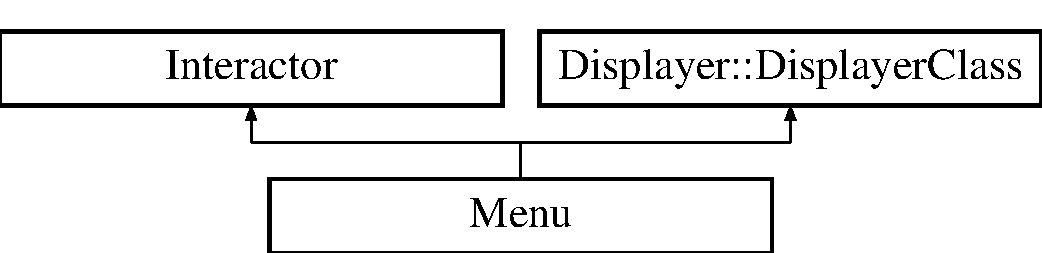
\includegraphics[height=2.000000cm]{class_menu}
\end{center}
\end{figure}
\subsubsection*{Public Member Functions}
\begin{DoxyCompactItemize}
\item 
virtual void \hyperlink{class_menu_ab19f32f8deac0f6c6960f04be8612067}{show\+Menu} ()
\item 
virtual void \hyperlink{class_menu_a2243881fe17494a0f6fc38a9211715d6}{get\+Choice} ()
\end{DoxyCompactItemize}
\subsubsection*{Private Member Functions}
\begin{DoxyCompactItemize}
\item 
virtual void \hyperlink{class_menu_a616bae73f48b58a1b5629354826c30cc}{display\+Message} (string message)
\item 
virtual void \hyperlink{class_menu_a3fbf0f02d6875bc41c4ee42597d99ff1}{check\+Matrix} (\hyperlink{classt_matrix}{t\+Matrix} $\ast$transition)
\item 
virtual void \hyperlink{class_menu_aad01d0f840a8be08e301d24d17b00b96}{parse\+Choice} ()
\item 
virtual void \hyperlink{class_menu_afd50901663e9f9b1210ba9ef7512c02d}{exit\+Program} ()
\item 
virtual string \hyperlink{class_menu_ab5b08e13a2db9ae41ac9e9696473a143}{get\+Suffix} ()
\item 
virtual bool \hyperlink{class_menu_ac759d0525a0736f421e8dfd443b1177c}{get\+Iterator\+Params} (\hyperlink{class_iterator_a1eb24c519953c2a333ea4a345b0c679c}{Iterator\+::\+Iterator\+Status} \&status, \hyperlink{class_iterator_a68bc1c5e7ad39ed78690beaa8a607430}{Iterator\+::\+Random\+Types} \&type, string \&file\+Name, string \&suffix, int \&num\+Of\+Genes)
\item 
virtual void \hyperlink{class_menu_a893fd3c7d9e4bc5e32d4e2e20d8da804}{get\+Simulator\+Params} (int \&num\+Of\+Genes, int \&simulate\+Type, string \&suffix)
\item 
virtual void \hyperlink{class_menu_a27538c5e2650251e98ed91257b0a2ba8}{test\+All\+On\+Simulator} ()
\item 
virtual void \hyperlink{class_menu_a4ff4dfbd63a558ed2a6aa79fbde05eba}{test\+All\+On\+Iterator} (\hyperlink{class_iterator_a1eb24c519953c2a333ea4a345b0c679c}{Iterator\+::\+Iterator\+Status} status)
\end{DoxyCompactItemize}
\subsubsection*{Additional Inherited Members}


\subsubsection{Detailed Description}
This is a concrete controller class for the application. 

This class is a subclass of the \char`\"{}\+Interactor\char`\"{} that also implements the \char`\"{}\+Displayer\char`\"{} interface. This class serves as a controller that gets user choice using \char`\"{}\+Displayer\char`\"{} interface methods and process it using \char`\"{}\+Interactor\char`\"{} class methods. 

\subsubsection{Member Function Documentation}
\hypertarget{class_menu_a3fbf0f02d6875bc41c4ee42597d99ff1}{\index{Menu@{Menu}!check\+Matrix@{check\+Matrix}}
\index{check\+Matrix@{check\+Matrix}!Menu@{Menu}}
\paragraph[{check\+Matrix}]{\setlength{\rightskip}{0pt plus 5cm}void Menu\+::check\+Matrix (
\begin{DoxyParamCaption}
\item[{{\bf t\+Matrix} $\ast$}]{transition}
\end{DoxyParamCaption}
)\hspace{0.3cm}{\ttfamily [private]}, {\ttfamily [virtual]}}}\label{class_menu_a3fbf0f02d6875bc41c4ee42597d99ff1}
Prints the transition matrix to standard output and ask the user to ensure the correctness of the matrix. 
\begin{DoxyParams}{Parameters}
{\em transition} & A pointer reference to the matrix to be checked. \\
\hline
\end{DoxyParams}


Implements \hyperlink{class_displayer_1_1_displayer_class_a9b9ea4661b05a211763792e392f3cdd5}{Displayer\+::\+Displayer\+Class}.

\hypertarget{class_menu_a616bae73f48b58a1b5629354826c30cc}{\index{Menu@{Menu}!display\+Message@{display\+Message}}
\index{display\+Message@{display\+Message}!Menu@{Menu}}
\paragraph[{display\+Message}]{\setlength{\rightskip}{0pt plus 5cm}virtual void Menu\+::display\+Message (
\begin{DoxyParamCaption}
\item[{string}]{message}
\end{DoxyParamCaption}
)\hspace{0.3cm}{\ttfamily [private]}, {\ttfamily [virtual]}}}\label{class_menu_a616bae73f48b58a1b5629354826c30cc}
Specific implementation of abstract method in \char`\"{}\+Displayer\char`\"{} interface. This method prints a message to console output. 
\begin{DoxyParams}{Parameters}
{\em message} & The message to be shown. \\
\hline
\end{DoxyParams}


Implements \hyperlink{class_displayer_1_1_displayer_class_ae572acc400418de40d2977a7b5556d45}{Displayer\+::\+Displayer\+Class}.

\hypertarget{class_menu_afd50901663e9f9b1210ba9ef7512c02d}{\index{Menu@{Menu}!exit\+Program@{exit\+Program}}
\index{exit\+Program@{exit\+Program}!Menu@{Menu}}
\paragraph[{exit\+Program}]{\setlength{\rightskip}{0pt plus 5cm}void Menu\+::exit\+Program (
\begin{DoxyParamCaption}
{}
\end{DoxyParamCaption}
)\hspace{0.3cm}{\ttfamily [private]}, {\ttfamily [virtual]}}}\label{class_menu_afd50901663e9f9b1210ba9ef7512c02d}
Display a \char`\"{}\+Process Complete\char`\"{} message then directly exit the program. 

Implements \hyperlink{class_displayer_1_1_displayer_class_a1ae1ffba6ab3b1effad2b042e2868ac4}{Displayer\+::\+Displayer\+Class}.

\hypertarget{class_menu_a2243881fe17494a0f6fc38a9211715d6}{\index{Menu@{Menu}!get\+Choice@{get\+Choice}}
\index{get\+Choice@{get\+Choice}!Menu@{Menu}}
\paragraph[{get\+Choice}]{\setlength{\rightskip}{0pt plus 5cm}void Menu\+::get\+Choice (
\begin{DoxyParamCaption}
{}
\end{DoxyParamCaption}
)\hspace{0.3cm}{\ttfamily [virtual]}}}\label{class_menu_a2243881fe17494a0f6fc38a9211715d6}
Get the choice from the user by taking in input from c++ standard keyboard input. 

Implements \hyperlink{class_displayer_1_1_displayer_class_ac61f3852eda7fe91a189927d33d4aef5}{Displayer\+::\+Displayer\+Class}.

\hypertarget{class_menu_ac759d0525a0736f421e8dfd443b1177c}{\index{Menu@{Menu}!get\+Iterator\+Params@{get\+Iterator\+Params}}
\index{get\+Iterator\+Params@{get\+Iterator\+Params}!Menu@{Menu}}
\paragraph[{get\+Iterator\+Params}]{\setlength{\rightskip}{0pt plus 5cm}bool Menu\+::get\+Iterator\+Params (
\begin{DoxyParamCaption}
\item[{{\bf Iterator\+::\+Iterator\+Status} \&}]{status, }
\item[{{\bf Iterator\+::\+Random\+Types} \&}]{type, }
\item[{string \&}]{file\+Name, }
\item[{string \&}]{suffix, }
\item[{int \&}]{num\+Of\+Genes}
\end{DoxyParamCaption}
)\hspace{0.3cm}{\ttfamily [private]}, {\ttfamily [virtual]}}}\label{class_menu_ac759d0525a0736f421e8dfd443b1177c}
Get the necessary parameters for initializing an \char`\"{}\+Iterator\char`\"{} instance. Information will be prompted to user from standard output.


\begin{DoxyParams}{Parameters}
{\em status} & Status of the \char`\"{}\+Iterator\char`\"{}, can be \char`\"{}\+P\+R\+O\+V\+I\+D\+E\+D\char`\"{} or \char`\"{}\+S\+I\+M\+U\+L\+A\+T\+E\+D\char`\"{}; \\
\hline
{\em type} & Type of algorithms used for decomposition; \\
\hline
{\em file\+Name} & The file name of the file storing the transition matrix; \\
\hline
{\em suffix} & Suffix obtained from user; \\
\hline
{\em num\+Of\+Genes} & The number of genes corresponding to the file with {\itshape  file\+Name } \\
\hline
\end{DoxyParams}
\begin{DoxyReturn}{Returns}
{\itshape \char`\"{}\+True\char`\"{}} if the \char`\"{}\+Iterator\char`\"{} is initialized in \char`\"{}\+Default\char`\"{} mode.
\end{DoxyReturn}
\begin{DoxyNote}{Note}
This function is an implementation of a function prototype from \char`\"{}\+Interactor\char`\"{} class. Implementation should be different depending on different types of user interaction. This is how it is used \+: 
\begin{DoxyCode}
\textcolor{keywordflow}{if} (\hyperlink{class_menu_ac759d0525a0736f421e8dfd443b1177c}{getIteratorParams}(status, type, fileName, suffix, numOfGenes))\{
    myIterator = \textcolor{keyword}{new} \hyperlink{class_iterator}{Iterator}();
\}\textcolor{keywordflow}{else}\{
     myIterator = \textcolor{keyword}{new} \hyperlink{class_iterator}{Iterator}(status, type);
\}
\hyperlink{class_interactor_ab67e4ff9ff5d44ee2001e7700dfeb164}{initializeIterator}(suffix, fileName, numOfGenes);
\end{DoxyCode}

\end{DoxyNote}
\begin{DoxySeeAlso}{See Also}
\hyperlink{class_interactor_aeb10be4d589b66a8624d7221f7600f87}{Interactor\+::initialize\+Iterator(string, string, int)}.
\end{DoxySeeAlso}
\begin{DoxyWarning}{Warning}
This method must be implemented, or the initialization process cannot complete. 
\end{DoxyWarning}


Implements \hyperlink{class_interactor_a6e98daf626d09b585375eec2d5311f25}{Interactor}.

\hypertarget{class_menu_a893fd3c7d9e4bc5e32d4e2e20d8da804}{\index{Menu@{Menu}!get\+Simulator\+Params@{get\+Simulator\+Params}}
\index{get\+Simulator\+Params@{get\+Simulator\+Params}!Menu@{Menu}}
\paragraph[{get\+Simulator\+Params}]{\setlength{\rightskip}{0pt plus 5cm}void Menu\+::get\+Simulator\+Params (
\begin{DoxyParamCaption}
\item[{int \&}]{num\+Of\+Genes, }
\item[{int \&}]{simulate\+Type, }
\item[{string \&}]{suffix}
\end{DoxyParamCaption}
)\hspace{0.3cm}{\ttfamily [private]}, {\ttfamily [virtual]}}}\label{class_menu_a893fd3c7d9e4bc5e32d4e2e20d8da804}
Get the necessary parameters for initializing a \char`\"{}\+Simulator\char`\"{} instance. Information will be prompted to user from standard output.


\begin{DoxyParams}{Parameters}
{\em num\+Of\+Genes} & The number of genes to simulate. \\
\hline
{\em simulate\+Type} & The type for simulation, either S\+P\+R\+A\+S\+E or F\+O\+R\+W\+A\+R\+D. \\
\hline
{\em suffix} & The file suffix added to the end of the output files. Implementation should be different depending on different types of user interaction. This is how it is used \+: 
\begin{DoxyCode}
\textcolor{keywordtype}{int} numOfGenes, simulateType;
\textcolor{keywordtype}{string} suffix;
\hyperlink{class_menu_a893fd3c7d9e4bc5e32d4e2e20d8da804}{getSimulatorParams}(numOfGenes, simulateType, suffix);
\hyperlink{class_interactor_a8416bb98d11e11b841db245e93c98853}{initializeSimulator}(numOfGenes, simulateType, suffix);
\end{DoxyCode}
\\
\hline
\end{DoxyParams}
\begin{DoxySeeAlso}{See Also}
\hyperlink{class_interactor_a1a9260b3dbc1c1f87933f98fadedb979}{Interactor\+::initialize\+Simulator(int, int, string)}.
\end{DoxySeeAlso}
\begin{DoxyWarning}{Warning}
This method must be implemented, or the initialization process cannot complete. 
\end{DoxyWarning}


Implements \hyperlink{class_interactor_a63d581b5afbf258b25915b318c1216c7}{Interactor}.

\hypertarget{class_menu_ab5b08e13a2db9ae41ac9e9696473a143}{\index{Menu@{Menu}!get\+Suffix@{get\+Suffix}}
\index{get\+Suffix@{get\+Suffix}!Menu@{Menu}}
\paragraph[{get\+Suffix}]{\setlength{\rightskip}{0pt plus 5cm}string Menu\+::get\+Suffix (
\begin{DoxyParamCaption}
{}
\end{DoxyParamCaption}
)\hspace{0.3cm}{\ttfamily [private]}, {\ttfamily [virtual]}}}\label{class_menu_ab5b08e13a2db9ae41ac9e9696473a143}
Get the file suffix from user by prompting a message to standard output. \begin{DoxyReturn}{Returns}
The suffix entered by the user. 
\end{DoxyReturn}


Implements \hyperlink{class_interactor_af3d8accfc60634bf82be9c438c0b9400}{Interactor}.

\hypertarget{class_menu_aad01d0f840a8be08e301d24d17b00b96}{\index{Menu@{Menu}!parse\+Choice@{parse\+Choice}}
\index{parse\+Choice@{parse\+Choice}!Menu@{Menu}}
\paragraph[{parse\+Choice}]{\setlength{\rightskip}{0pt plus 5cm}void Menu\+::parse\+Choice (
\begin{DoxyParamCaption}
{}
\end{DoxyParamCaption}
)\hspace{0.3cm}{\ttfamily [private]}, {\ttfamily [virtual]}}}\label{class_menu_aad01d0f840a8be08e301d24d17b00b96}
A method to parse the choice from user. Deciding which mehod to call upon each choice. 

Implements \hyperlink{class_displayer_1_1_displayer_class_a84478e90e6895f0061268c59d2040cc4}{Displayer\+::\+Displayer\+Class}.

\hypertarget{class_menu_ab19f32f8deac0f6c6960f04be8612067}{\index{Menu@{Menu}!show\+Menu@{show\+Menu}}
\index{show\+Menu@{show\+Menu}!Menu@{Menu}}
\paragraph[{show\+Menu}]{\setlength{\rightskip}{0pt plus 5cm}void Menu\+::show\+Menu (
\begin{DoxyParamCaption}
{}
\end{DoxyParamCaption}
)\hspace{0.3cm}{\ttfamily [virtual]}}}\label{class_menu_ab19f32f8deac0f6c6960f04be8612067}
The method that shows the menu to user. This implementation will print the menu to the console output. The information of the menu is stored in the namespace \char`\"{}\+Displayer\char`\"{}. 

Implements \hyperlink{class_displayer_1_1_displayer_class_aa259ca88fafe20ad118cb8a492c88351}{Displayer\+::\+Displayer\+Class}.

\hypertarget{class_menu_a4ff4dfbd63a558ed2a6aa79fbde05eba}{\index{Menu@{Menu}!test\+All\+On\+Iterator@{test\+All\+On\+Iterator}}
\index{test\+All\+On\+Iterator@{test\+All\+On\+Iterator}!Menu@{Menu}}
\paragraph[{test\+All\+On\+Iterator}]{\setlength{\rightskip}{0pt plus 5cm}void Menu\+::test\+All\+On\+Iterator (
\begin{DoxyParamCaption}
\item[{{\bf Iterator\+::\+Iterator\+Status}}]{status}
\end{DoxyParamCaption}
)\hspace{0.3cm}{\ttfamily [private]}, {\ttfamily [virtual]}}}\label{class_menu_a4ff4dfbd63a558ed2a6aa79fbde05eba}
Test all prepared iteration cases, either P\+R\+O\+V\+I\+D\+E\+D or S\+I\+M\+U\+L\+A\+T\+E\+D 
\begin{DoxyParams}{Parameters}
{\em status} & Input file type. P\+R\+O\+V\+I\+D\+E\+D or S\+I\+M\+U\+L\+A\+T\+E\+D. \\
\hline
\end{DoxyParams}


Implements \hyperlink{class_interactor_aeeec69df23673e87530a1b1db98998ee}{Interactor}.

\hypertarget{class_menu_a27538c5e2650251e98ed91257b0a2ba8}{\index{Menu@{Menu}!test\+All\+On\+Simulator@{test\+All\+On\+Simulator}}
\index{test\+All\+On\+Simulator@{test\+All\+On\+Simulator}!Menu@{Menu}}
\paragraph[{test\+All\+On\+Simulator}]{\setlength{\rightskip}{0pt plus 5cm}void Menu\+::test\+All\+On\+Simulator (
\begin{DoxyParamCaption}
{}
\end{DoxyParamCaption}
)\hspace{0.3cm}{\ttfamily [private]}, {\ttfamily [virtual]}}}\label{class_menu_a27538c5e2650251e98ed91257b0a2ba8}
Test all prepared simulation cases. 

Implements \hyperlink{class_interactor_ac2282b0725d5bd6216edb0f2ea4dd421}{Interactor}.



The documentation for this class was generated from the following files\+:\begin{DoxyCompactItemize}
\item 
\hyperlink{_menu_8h}{Menu.\+h}\item 
Menu.\+cpp\end{DoxyCompactItemize}

\hypertarget{classr_matrix}{\subsection{r\+Matrix Class Reference}
\label{classr_matrix}\index{r\+Matrix@{r\+Matrix}}
}


This class holds the data needed for representing a boolean matrix.  




{\ttfamily \#include $<$r\+Matrix.\+h$>$}

Inheritance diagram for r\+Matrix\+:\begin{figure}[H]
\begin{center}
\leavevmode
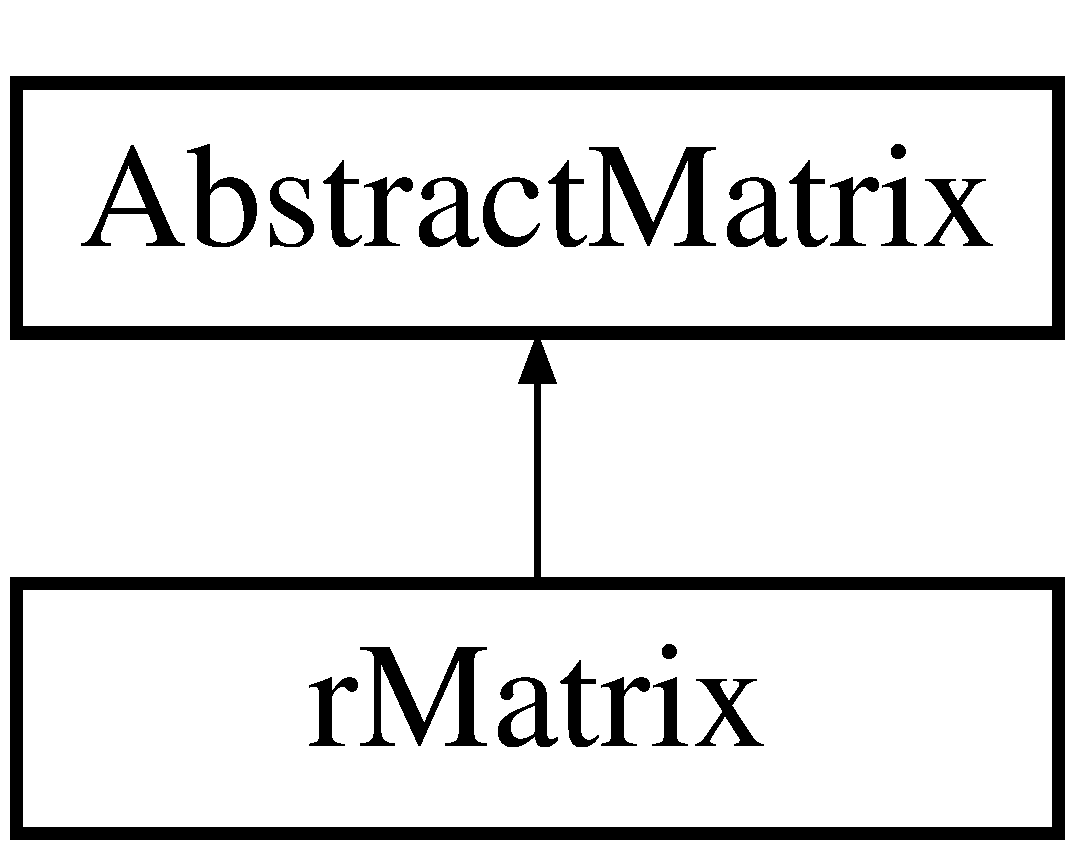
\includegraphics[height=2.000000cm]{classr_matrix}
\end{center}
\end{figure}
\subsubsection*{Public Member Functions}
\begin{DoxyCompactItemize}
\item 
\hyperlink{classr_matrix_afb32c7699d7dff3dd143f42ab42d09d4}{r\+Matrix} (int n=1)
\item 
\hyperlink{classr_matrix_a2a4aff28e459377c12b3d818fd26374c}{r\+Matrix} (vector$<$ int $>$ \&positions)
\item 
virtual void \hyperlink{classr_matrix_a2a22671198a516a8165306d5406e539b}{print} (ostream \&output)
\end{DoxyCompactItemize}
\subsubsection*{Private Attributes}
\begin{DoxyCompactItemize}
\item 
\hypertarget{classr_matrix_a88d428b77fd5dbecaf0e852cfe84547b}{vector$<$ int $>$ \hyperlink{classr_matrix_a88d428b77fd5dbecaf0e852cfe84547b}{matrix}}\label{classr_matrix_a88d428b77fd5dbecaf0e852cfe84547b}

\begin{DoxyCompactList}\small\item\em A vector$<$int$>$ storing the positions of ones in each column. \end{DoxyCompactList}\end{DoxyCompactItemize}
\subsubsection*{Additional Inherited Members}


\subsubsection{Detailed Description}
This class holds the data needed for representing a boolean matrix. 

The instances of this class can be initiated with number of genes, and a vector of rows. It also implements the print method. 

\subsubsection{Constructor \& Destructor Documentation}
\hypertarget{classr_matrix_afb32c7699d7dff3dd143f42ab42d09d4}{\index{r\+Matrix@{r\+Matrix}!r\+Matrix@{r\+Matrix}}
\index{r\+Matrix@{r\+Matrix}!r\+Matrix@{r\+Matrix}}
\paragraph[{r\+Matrix}]{\setlength{\rightskip}{0pt plus 5cm}r\+Matrix\+::r\+Matrix (
\begin{DoxyParamCaption}
\item[{int}]{n = {\ttfamily 1}}
\end{DoxyParamCaption}
)}}\label{classr_matrix_afb32c7699d7dff3dd143f42ab42d09d4}
Default constructor, creates an instance with random positions of ones. \hypertarget{classr_matrix_a2a4aff28e459377c12b3d818fd26374c}{\index{r\+Matrix@{r\+Matrix}!r\+Matrix@{r\+Matrix}}
\index{r\+Matrix@{r\+Matrix}!r\+Matrix@{r\+Matrix}}
\paragraph[{r\+Matrix}]{\setlength{\rightskip}{0pt plus 5cm}r\+Matrix\+::r\+Matrix (
\begin{DoxyParamCaption}
\item[{vector$<$ int $>$ \&}]{positions}
\end{DoxyParamCaption}
)}}\label{classr_matrix_a2a4aff28e459377c12b3d818fd26374c}
This constructor takes in a vector$<$int$>$ as an input and generate and instance of boolean matrix with the corresponding row positions being one. 

\subsubsection{Member Function Documentation}
\hypertarget{classr_matrix_a2a22671198a516a8165306d5406e539b}{\index{r\+Matrix@{r\+Matrix}!print@{print}}
\index{print@{print}!r\+Matrix@{r\+Matrix}}
\paragraph[{print}]{\setlength{\rightskip}{0pt plus 5cm}void r\+Matrix\+::print (
\begin{DoxyParamCaption}
\item[{ostream \&}]{output}
\end{DoxyParamCaption}
)\hspace{0.3cm}{\ttfamily [virtual]}}}\label{classr_matrix_a2a22671198a516a8165306d5406e539b}
Print the matrix in a n by n matrix form to the output stream 
\begin{DoxyParams}{Parameters}
{\em output} & The stream for output \\
\hline
\end{DoxyParams}


Implements \hyperlink{class_abstract_matrix_a300f90398cb2bac75c8d2ab56bdde1ab}{Abstract\+Matrix}.



The documentation for this class was generated from the following files\+:\begin{DoxyCompactItemize}
\item 
\hyperlink{r_matrix_8h}{r\+Matrix.\+h}\item 
r\+Matrix.\+cpp\end{DoxyCompactItemize}

\hypertarget{class_simulator}{\subsection{Simulator Class Reference}
\label{class_simulator}\index{Simulator@{Simulator}}
}


This is a class that handles simulation process.  




{\ttfamily \#include $<$Simulator.\+h$>$}

Inheritance diagram for Simulator\+:\begin{figure}[H]
\begin{center}
\leavevmode
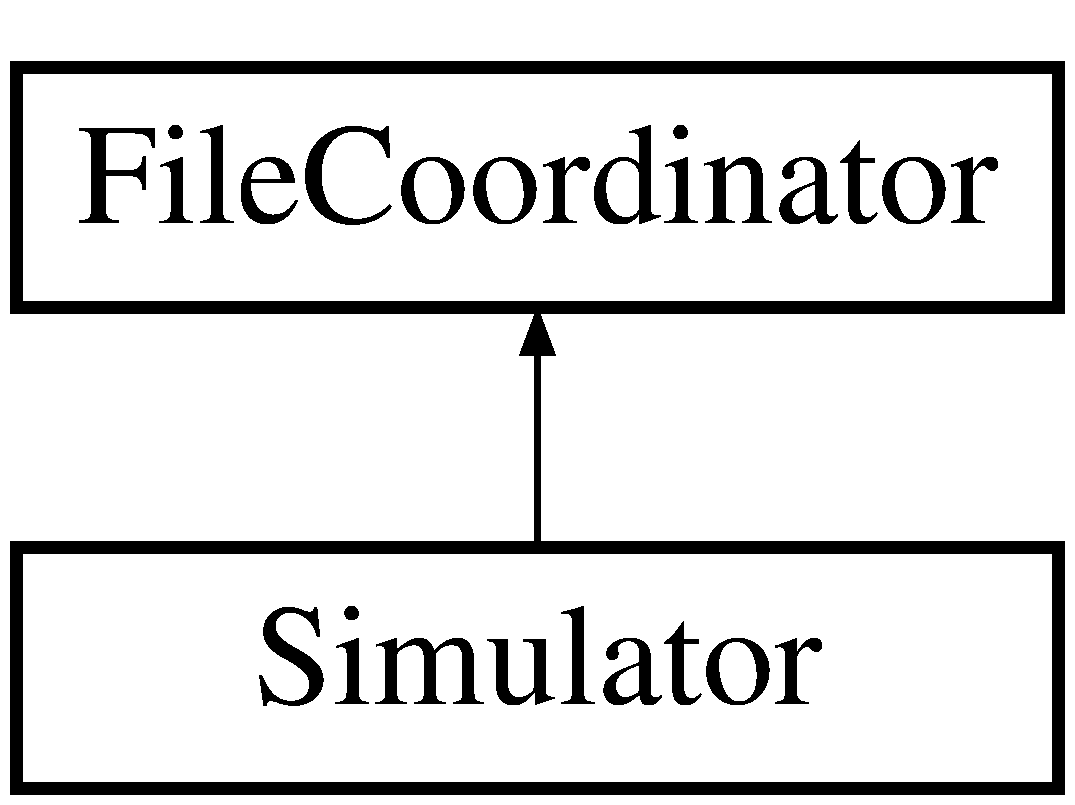
\includegraphics[height=2.000000cm]{class_simulator}
\end{center}
\end{figure}
\subsubsection*{Public Member Functions}
\begin{DoxyCompactItemize}
\item 
string \hyperlink{class_simulator_a252d919d45b1789b7fa809e8ac6d8c63}{simulate} ()
\end{DoxyCompactItemize}
\subsubsection*{Private Member Functions}
\begin{DoxyCompactItemize}
\item 
void \hyperlink{class_simulator_ab05f5807293d42624526d1f3fe6aab71}{generate\+Transition} (int n)
\item 
void \hyperlink{class_simulator_aced31482cc73fa28ac9067325c9dd185}{generate\+Transition} (int n, int m, ostream \&output)
\item 
virtual string \hyperlink{class_simulator_a1270d2e2eeaa4aa3284e2d74a8644bc3}{save\+Matrix} ()
\end{DoxyCompactItemize}
\subsubsection*{Additional Inherited Members}


\subsubsection{Detailed Description}
This is a class that handles simulation process. 

The \hyperlink{class_simulator}{Simulator} class serves to simulate transition matrix with a given number of genes. There are two types of simulation\+: S\+P\+A\+R\+S\+E and F\+O\+R\+W\+A\+R\+D. The S\+P\+A\+R\+S\+E simulation will control the number of non-\/zero entries in each column below the number of genes.

The F\+O\+R\+W\+A\+R\+D simulation will simulate 10 B\+Ns and their corresponding weights and construct a final transition matrix. But the result of this simulation is not guaranteed to be sparse, especially when the number of genes are small. 

\subsubsection{Member Function Documentation}
\hypertarget{class_simulator_ab05f5807293d42624526d1f3fe6aab71}{\index{Simulator@{Simulator}!generate\+Transition@{generate\+Transition}}
\index{generate\+Transition@{generate\+Transition}!Simulator@{Simulator}}
\paragraph[{generate\+Transition}]{\setlength{\rightskip}{0pt plus 5cm}void Simulator\+::generate\+Transition (
\begin{DoxyParamCaption}
\item[{int}]{n}
\end{DoxyParamCaption}
)\hspace{0.3cm}{\ttfamily [private]}}}\label{class_simulator_ab05f5807293d42624526d1f3fe6aab71}
The method for generating S\+P\+A\+R\+S\+E transition matrix. 
\begin{DoxyParams}{Parameters}
{\em n} & The number of genes to simulate \\
\hline
\end{DoxyParams}
\hypertarget{class_simulator_aced31482cc73fa28ac9067325c9dd185}{\index{Simulator@{Simulator}!generate\+Transition@{generate\+Transition}}
\index{generate\+Transition@{generate\+Transition}!Simulator@{Simulator}}
\paragraph[{generate\+Transition}]{\setlength{\rightskip}{0pt plus 5cm}void Simulator\+::generate\+Transition (
\begin{DoxyParamCaption}
\item[{int}]{n, }
\item[{int}]{m, }
\item[{ostream \&}]{output}
\end{DoxyParamCaption}
)\hspace{0.3cm}{\ttfamily [private]}}}\label{class_simulator_aced31482cc73fa28ac9067325c9dd185}
The method for generating F\+O\+R\+W\+A\+R\+D transition matrix. 
\begin{DoxyParams}{Parameters}
{\em n} & The number of genes to simulate \\
\hline
{\em m} & The number of B\+Ns used in simulation. The default value is 10 \\
\hline
{\em output} & An output stream to save the B\+Ns and their weights \\
\hline
\end{DoxyParams}
\hypertarget{class_simulator_a1270d2e2eeaa4aa3284e2d74a8644bc3}{\index{Simulator@{Simulator}!save\+Matrix@{save\+Matrix}}
\index{save\+Matrix@{save\+Matrix}!Simulator@{Simulator}}
\paragraph[{save\+Matrix}]{\setlength{\rightskip}{0pt plus 5cm}string Simulator\+::save\+Matrix (
\begin{DoxyParamCaption}
{}
\end{DoxyParamCaption}
)\hspace{0.3cm}{\ttfamily [private]}, {\ttfamily [virtual]}}}\label{class_simulator_a1270d2e2eeaa4aa3284e2d74a8644bc3}
Saves the transition matrix to current file. \begin{DoxyReturn}{Returns}
Returns the full path of the file. 
\end{DoxyReturn}


Reimplemented from \hyperlink{class_file_coordinator_a913c584fd94fdcacd120bf6f52819aad}{File\+Coordinator}.

\hypertarget{class_simulator_a252d919d45b1789b7fa809e8ac6d8c63}{\index{Simulator@{Simulator}!simulate@{simulate}}
\index{simulate@{simulate}!Simulator@{Simulator}}
\paragraph[{simulate}]{\setlength{\rightskip}{0pt plus 5cm}string Simulator\+::simulate (
\begin{DoxyParamCaption}
{}
\end{DoxyParamCaption}
)}}\label{class_simulator_a252d919d45b1789b7fa809e8ac6d8c63}
The main method available for clients. After setting the number of genes and type of simulation, the client needs only to call this method to simulate and save results in output files. \begin{DoxyReturn}{Returns}
A message indicating location and type of simulation.
\end{DoxyReturn}
\begin{DoxySeeAlso}{See Also}
\hyperlink{class_interactor_a60a3be74e1e954f23182fab7b638164e}{Interactor\+::start\+Simulator} 
\end{DoxySeeAlso}


The documentation for this class was generated from the following files\+:\begin{DoxyCompactItemize}
\item 
\hyperlink{_simulator_8h}{Simulator.\+h}\item 
Simulator.\+cpp\end{DoxyCompactItemize}

\hypertarget{classt_matrix}{\subsection{t\+Matrix Class Reference}
\label{classt_matrix}\index{t\+Matrix@{t\+Matrix}}
}


Internal data structure representing a matrix that has constant column sums.  




{\ttfamily \#include $<$t\+Matrix.\+h$>$}

Inheritance diagram for t\+Matrix\+:\begin{figure}[H]
\begin{center}
\leavevmode
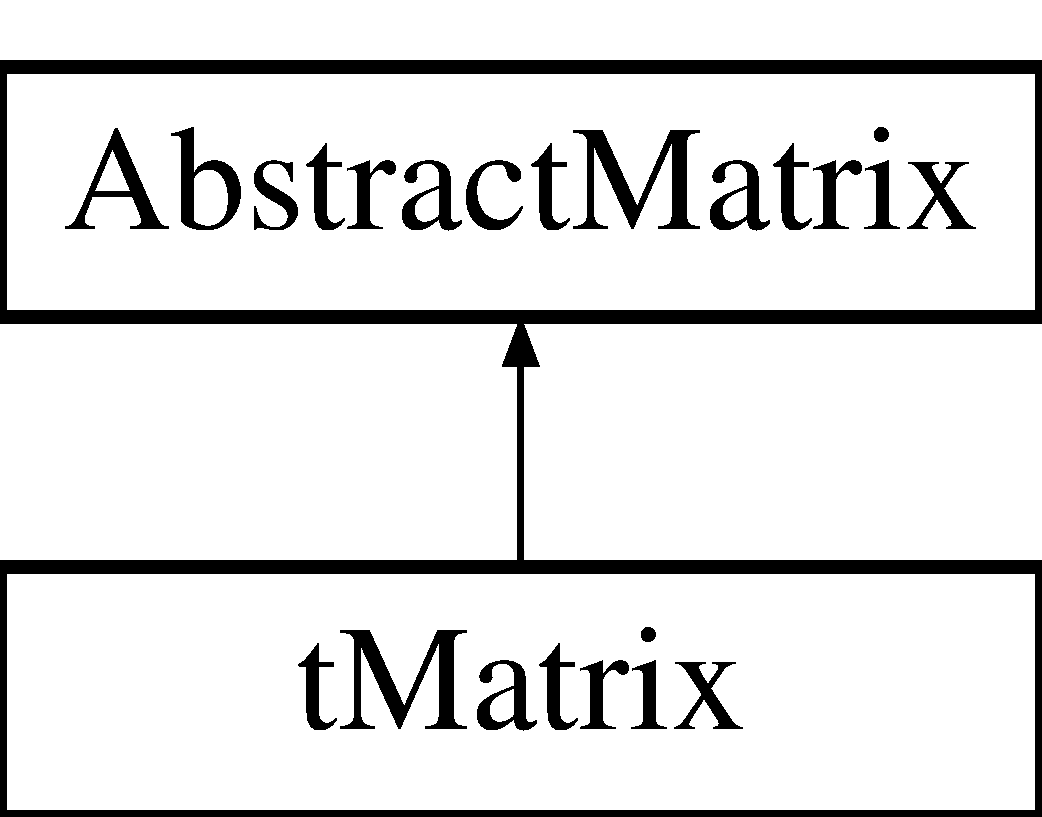
\includegraphics[height=2.000000cm]{classt_matrix}
\end{center}
\end{figure}
\subsubsection*{Public Member Functions}
\begin{DoxyCompactItemize}
\item 
\hyperlink{classt_matrix_a58e483fc473143ff57c2d821caf047e4}{t\+Matrix} (const \hyperlink{classr_matrix}{r\+Matrix} \&base)
\item 
double \hyperlink{classt_matrix_a98e50b73500855a69245ca57303085b1}{module} ()
\item 
void \hyperlink{classt_matrix_a52d5417362388c95db488ee6c8e008fa}{set} (int i, int j, double value)
\item 
map$<$ int, double $>$ \hyperlink{classt_matrix_a403a16974063512eb8c384f4b681d946}{get} (int col) const 
\item 
\hyperlink{classt_matrix}{t\+Matrix} \& \hyperlink{classt_matrix_a4308bb70d63f0301ca2e1fcacac77beb}{operator+=} (const \hyperlink{classt_matrix}{t\+Matrix} \&rhs)
\item 
virtual void \hyperlink{classt_matrix_a7e1b5623978bf16ace999ce22a28d350}{print} (ostream \&output)
\end{DoxyCompactItemize}
\subsubsection*{Static Public Member Functions}
\begin{DoxyCompactItemize}
\item 
static \hyperlink{classt_matrix}{t\+Matrix} \hyperlink{classt_matrix_aa782f22b376682aca4fd61ac9e6358e5}{times} (\hyperlink{classr_matrix}{r\+Matrix} lhs, const double k)
\end{DoxyCompactItemize}
\subsubsection*{Private Attributes}
\begin{DoxyCompactItemize}
\item 
vector$<$ map$<$ int, double $>$ $>$ \hyperlink{classt_matrix_a3d962506eec7f8d0f65cb2d50e5b81bc}{matrix}
\end{DoxyCompactItemize}
\subsubsection*{Additional Inherited Members}


\subsubsection{Detailed Description}
Internal data structure representing a matrix that has constant column sums. 

This matrix inherit the \char`\"{}print\char`\"{} method from \hyperlink{class_abstract_matrix}{Abstract\+Matrix} to print the matrix as $n\times n$ matrix to an output stream. 

\subsubsection{Constructor \& Destructor Documentation}
\hypertarget{classt_matrix_a58e483fc473143ff57c2d821caf047e4}{\index{t\+Matrix@{t\+Matrix}!t\+Matrix@{t\+Matrix}}
\index{t\+Matrix@{t\+Matrix}!t\+Matrix@{t\+Matrix}}
\paragraph[{t\+Matrix}]{\setlength{\rightskip}{0pt plus 5cm}t\+Matrix\+::t\+Matrix (
\begin{DoxyParamCaption}
\item[{const {\bf r\+Matrix} \&}]{base}
\end{DoxyParamCaption}
)}}\label{classt_matrix_a58e483fc473143ff57c2d821caf047e4}
Construct a \hyperlink{classt_matrix}{t\+Matrix} using an \hyperlink{classr_matrix}{r\+Matrix} instance. The matrices are the same, but this instance supports \hyperlink{classt_matrix}{t\+Matrix} operations.

\begin{DoxyNote}{Note}
Typical usage \+: \hyperlink{classt_matrix}{t\+Matrix} transition(\+R); 
\end{DoxyNote}


\subsubsection{Member Function Documentation}
\hypertarget{classt_matrix_a403a16974063512eb8c384f4b681d946}{\index{t\+Matrix@{t\+Matrix}!get@{get}}
\index{get@{get}!t\+Matrix@{t\+Matrix}}
\paragraph[{get}]{\setlength{\rightskip}{0pt plus 5cm}map$<$ int, double $>$ t\+Matrix\+::get (
\begin{DoxyParamCaption}
\item[{int}]{col}
\end{DoxyParamCaption}
) const}}\label{classt_matrix_a403a16974063512eb8c384f4b681d946}
Get the colth column of the matrix. 
\begin{DoxyParams}{Parameters}
{\em col} & Column number; \\
\hline
\end{DoxyParams}
\begin{DoxyReturn}{Returns}
The colth column as a map from int to double 
\end{DoxyReturn}
\hypertarget{classt_matrix_a98e50b73500855a69245ca57303085b1}{\index{t\+Matrix@{t\+Matrix}!module@{module}}
\index{module@{module}!t\+Matrix@{t\+Matrix}}
\paragraph[{module}]{\setlength{\rightskip}{0pt plus 5cm}double t\+Matrix\+::module (
\begin{DoxyParamCaption}
{}
\end{DoxyParamCaption}
)}}\label{classt_matrix_a98e50b73500855a69245ca57303085b1}
Calculates the Frobinous module of the matrix as \+: $ \sqrt{\sum_{i, j}{a_{ij}^2}}$.

\begin{DoxyReturn}{Returns}
The module of the matrix 
\end{DoxyReturn}
\hypertarget{classt_matrix_a4308bb70d63f0301ca2e1fcacac77beb}{\index{t\+Matrix@{t\+Matrix}!operator+=@{operator+=}}
\index{operator+=@{operator+=}!t\+Matrix@{t\+Matrix}}
\paragraph[{operator+=}]{\setlength{\rightskip}{0pt plus 5cm}{\bf t\+Matrix} \& t\+Matrix\+::operator+= (
\begin{DoxyParamCaption}
\item[{const {\bf t\+Matrix} \&}]{rhs}
\end{DoxyParamCaption}
)}}\label{classt_matrix_a4308bb70d63f0301ca2e1fcacac77beb}
Defines addition between transition matrices.

\begin{DoxyNote}{Note}
Typical usage \+:
\begin{DoxyCode}
transition += anotherTransition; 
\end{DoxyCode}
 
\end{DoxyNote}
\hypertarget{classt_matrix_a7e1b5623978bf16ace999ce22a28d350}{\index{t\+Matrix@{t\+Matrix}!print@{print}}
\index{print@{print}!t\+Matrix@{t\+Matrix}}
\paragraph[{print}]{\setlength{\rightskip}{0pt plus 5cm}void t\+Matrix\+::print (
\begin{DoxyParamCaption}
\item[{ostream \&}]{output}
\end{DoxyParamCaption}
)\hspace{0.3cm}{\ttfamily [virtual]}}}\label{classt_matrix_a7e1b5623978bf16ace999ce22a28d350}
Print the matrix in a n by n matrix form to the output stream 
\begin{DoxyParams}{Parameters}
{\em output} & The stream for output \\
\hline
\end{DoxyParams}


Implements \hyperlink{class_abstract_matrix_a300f90398cb2bac75c8d2ab56bdde1ab}{Abstract\+Matrix}.

\hypertarget{classt_matrix_a52d5417362388c95db488ee6c8e008fa}{\index{t\+Matrix@{t\+Matrix}!set@{set}}
\index{set@{set}!t\+Matrix@{t\+Matrix}}
\paragraph[{set}]{\setlength{\rightskip}{0pt plus 5cm}void t\+Matrix\+::set (
\begin{DoxyParamCaption}
\item[{int}]{i, }
\item[{int}]{j, }
\item[{double}]{value}
\end{DoxyParamCaption}
)}}\label{classt_matrix_a52d5417362388c95db488ee6c8e008fa}
Set the ith row jth column entry to the given value. 
\begin{DoxyParams}{Parameters}
{\em i} & Row number; \\
\hline
{\em j} & Column number; \\
\hline
{\em value} & The value to set. \\
\hline
\end{DoxyParams}
\hypertarget{classt_matrix_aa782f22b376682aca4fd61ac9e6358e5}{\index{t\+Matrix@{t\+Matrix}!times@{times}}
\index{times@{times}!t\+Matrix@{t\+Matrix}}
\paragraph[{times}]{\setlength{\rightskip}{0pt plus 5cm}{\bf t\+Matrix} t\+Matrix\+::times (
\begin{DoxyParamCaption}
\item[{{\bf r\+Matrix}}]{lhs, }
\item[{const double}]{k}
\end{DoxyParamCaption}
)\hspace{0.3cm}{\ttfamily [static]}}}\label{classt_matrix_aa782f22b376682aca4fd61ac9e6358e5}
Defines scalar multiplication on boolean matrix. 
\begin{DoxyParams}{Parameters}
{\em lhs} & The boolean matrix to multiply on; \\
\hline
{\em k} & The scalar; \\
\hline
\end{DoxyParams}
\begin{DoxyReturn}{Returns}
A \hyperlink{classt_matrix}{t\+Matrix} instance as the result of the scalar multiplication
\end{DoxyReturn}
\begin{DoxyNote}{Note}
Typical usage \+:
\begin{DoxyCode}
\hyperlink{classt_matrix}{tMatrix} transition = \hyperlink{classt_matrix_aa782f22b376682aca4fd61ac9e6358e5}{tMatrix::times}(R, k); 
\end{DoxyCode}
 
\end{DoxyNote}


\subsubsection{Member Data Documentation}
\hypertarget{classt_matrix_a3d962506eec7f8d0f65cb2d50e5b81bc}{\index{t\+Matrix@{t\+Matrix}!matrix@{matrix}}
\index{matrix@{matrix}!t\+Matrix@{t\+Matrix}}
\paragraph[{matrix}]{\setlength{\rightskip}{0pt plus 5cm}vector$<$map$<$int, double$>$ $>$ t\+Matrix\+::matrix\hspace{0.3cm}{\ttfamily [private]}}}\label{classt_matrix_a3d962506eec7f8d0f65cb2d50e5b81bc}
A vector of map$<$int, double$>$ storing the entries of the matrix. The matrix\mbox{[}j\mbox{]}\mbox{[}i\mbox{]} represents the (i, j)th entry of the matrix.

\begin{DoxyNote}{Note}
Only non-\/zero entries are stored, zero entries cannot be found in any of the maps. 
\end{DoxyNote}


The documentation for this class was generated from the following files\+:\begin{DoxyCompactItemize}
\item 
\hyperlink{t_matrix_8h}{t\+Matrix.\+h}\item 
t\+Matrix.\+cpp\end{DoxyCompactItemize}

\section{File Documentation}
\hypertarget{_abstract_matrix_8h}{\subsection{Abstract\+Matrix.\+h File Reference}
\label{_abstract_matrix_8h}\index{Abstract\+Matrix.\+h@{Abstract\+Matrix.\+h}}
}


This is an abstract class/interface for matrix.  


{\ttfamily \#include $<$iostream$>$}\\*
\subsubsection*{Classes}
\begin{DoxyCompactItemize}
\item 
class \hyperlink{class_abstract_matrix}{Abstract\+Matrix}
\begin{DoxyCompactList}\small\item\em This class defines some of the basic operations we need for our matrix. \end{DoxyCompactList}\end{DoxyCompactItemize}


\subsubsection{Detailed Description}
This is an abstract class/interface for matrix. 


\hypertarget{_displayer_8h}{\subsection{Displayer.\+h File Reference}
\label{_displayer_8h}\index{Displayer.\+h@{Displayer.\+h}}
}


This is an interface for the \char`\"{}\+View\char`\"{}.  


\subsubsection*{Classes}
\begin{DoxyCompactItemize}
\item 
class \hyperlink{class_displayer_1_1_displayer_class}{Displayer\+::\+Displayer\+Class}
\begin{DoxyCompactList}\small\item\em Abstract interface for direct interation with end users. \end{DoxyCompactList}\end{DoxyCompactItemize}


\subsubsection{Detailed Description}
This is an interface for the \char`\"{}\+View\char`\"{}. 

This interface abstracts methods needed for the \char`\"{}\+View\char`\"{}. Any controller class should implement this interface. Besides, the namespace Displayer also provides some interaction messages that could be presented to end users. 
\hypertarget{_file_coordinator_8h}{\subsection{File\+Coordinator.\+h File Reference}
\label{_file_coordinator_8h}\index{File\+Coordinator.\+h@{File\+Coordinator.\+h}}
}


An abstract class for file manipulation.  


{\ttfamily \#include $<$string$>$}\\*
{\ttfamily \#include $<$fstream$>$}\\*
{\ttfamily \#include \char`\"{}t\+Matrix.\+h\char`\"{}}\\*
\subsubsection*{Classes}
\begin{DoxyCompactItemize}
\item 
class \hyperlink{class_file_coordinator}{File\+Coordinator}
\begin{DoxyCompactList}\small\item\em Abstract class for file manipulations. \end{DoxyCompactList}\end{DoxyCompactItemize}


\subsubsection{Detailed Description}
An abstract class for file manipulation. 

This file contains the declaration of the abstract class responsible for file manipulation.

\begin{DoxyAuthor}{Author}
Liang Ruo\+Chen 
\end{DoxyAuthor}
\begin{DoxyVersion}{Version}
2.\+1 09/04/2014 
\end{DoxyVersion}

\hypertarget{_interactor_8h}{\subsection{Interactor.\+h File Reference}
\label{_interactor_8h}\index{Interactor.\+h@{Interactor.\+h}}
}


An abstract controller class.  


{\ttfamily \#include $<$iostream$>$}\\*
{\ttfamily \#include $<$string$>$}\\*
{\ttfamily \#include $<$stdlib.\+h$>$}\\*
{\ttfamily \#include \char`\"{}Simulator.\+h\char`\"{}}\\*
{\ttfamily \#include \char`\"{}Iterator.\+h\char`\"{}}\\*
\subsubsection*{Classes}
\begin{DoxyCompactItemize}
\item 
class \hyperlink{class_interactor}{Interactor}
\begin{DoxyCompactList}\small\item\em An abstract controller class that contains method prototypes or basic implementations of methods for further overriding. \end{DoxyCompactList}\end{DoxyCompactItemize}


\subsubsection{Detailed Description}
An abstract controller class. 

This controller has reference to \hyperlink{class_simulator}{Simulator} and \hyperlink{class_iterator}{Iterator} objects that do the background computation.

\begin{DoxyAuthor}{Author}
Vincent 
\end{DoxyAuthor}
\begin{DoxyVersion}{Version}
2.\+1 22/04/2014 
\end{DoxyVersion}

\hypertarget{_iterator_8h}{\subsection{Iterator.\+h File Reference}
\label{_iterator_8h}\index{Iterator.\+h@{Iterator.\+h}}
}


A file containing class definitions for \hyperlink{class_iterator}{Iterator}.  


{\ttfamily \#include \char`\"{}File\+Coordinator.\+h\char`\"{}}\\*
{\ttfamily \#include $<$set$>$}\\*
\subsubsection*{Classes}
\begin{DoxyCompactItemize}
\item 
class \hyperlink{class_iterator}{Iterator}
\begin{DoxyCompactList}\small\item\em This class encapsulates the functionality of an inverse iterator. \end{DoxyCompactList}\end{DoxyCompactItemize}


\subsubsection{Detailed Description}
A file containing class definitions for \hyperlink{class_iterator}{Iterator}. 

Apart from \hyperlink{class_iterator}{Iterator}, this file also includes definitions for Iterator\+Status and Random\+Types, which are important enumeration types for simulation and iteration. 
\hypertarget{_menu_8h}{\subsection{Menu.\+h File Reference}
\label{_menu_8h}\index{Menu.\+h@{Menu.\+h}}
}


This file contains declaration of the class \hyperlink{class_menu}{Menu}.  


{\ttfamily \#include \char`\"{}Interactor.\+h\char`\"{}}\\*
{\ttfamily \#include \char`\"{}Displayer.\+h\char`\"{}}\\*
\subsubsection*{Classes}
\begin{DoxyCompactItemize}
\item 
class \hyperlink{class_menu}{Menu}
\begin{DoxyCompactList}\small\item\em This is a concrete controller class for the application. \end{DoxyCompactList}\end{DoxyCompactItemize}


\subsubsection{Detailed Description}
This file contains declaration of the class \hyperlink{class_menu}{Menu}. 

\begin{DoxyAuthor}{Author}
Liang Ruo\+Chen 
\end{DoxyAuthor}
\begin{DoxyVersion}{Version}
2.\+1 09/04/2014 
\end{DoxyVersion}

\hypertarget{r_matrix_8h}{\subsection{r\+Matrix.\+h File Reference}
\label{r_matrix_8h}\index{r\+Matrix.\+h@{r\+Matrix.\+h}}
}


This is the boolean matrix class.  


{\ttfamily \#include \char`\"{}Abstract\+Matrix.\+h\char`\"{}}\\*
{\ttfamily \#include $<$vector$>$}\\*
\subsubsection*{Classes}
\begin{DoxyCompactItemize}
\item 
class \hyperlink{classr_matrix}{r\+Matrix}
\begin{DoxyCompactList}\small\item\em This class holds the data needed for representing a boolean matrix. \end{DoxyCompactList}\end{DoxyCompactItemize}


\subsubsection{Detailed Description}
This is the boolean matrix class. 

\begin{DoxyAuthor}{Author}
Liang Ruo\+Chen 
\end{DoxyAuthor}
\begin{DoxyVersion}{Version}
2.\+1 09/04/2014 
\end{DoxyVersion}

\hypertarget{_simulator_8h}{\subsection{Simulator.\+h File Reference}
\label{_simulator_8h}\index{Simulator.\+h@{Simulator.\+h}}
}


This file contains class definitions of \hyperlink{class_simulator}{Simulator} class.  


{\ttfamily \#include \char`\"{}File\+Coordinator.\+h\char`\"{}}\\*
\subsubsection*{Classes}
\begin{DoxyCompactItemize}
\item 
class \hyperlink{class_simulator}{Simulator}
\begin{DoxyCompactList}\small\item\em This is a class that handles simulation process. \end{DoxyCompactList}\end{DoxyCompactItemize}


\subsubsection{Detailed Description}
This file contains class definitions of \hyperlink{class_simulator}{Simulator} class. 


\hypertarget{t_matrix_8h}{\subsection{t\+Matrix.\+h File Reference}
\label{t_matrix_8h}\index{t\+Matrix.\+h@{t\+Matrix.\+h}}
}


This file contains declaration of transition matrix class.  


{\ttfamily \#include $<$map$>$}\\*
{\ttfamily \#include $<$iomanip$>$}\\*
{\ttfamily \#include \char`\"{}r\+Matrix.\+h\char`\"{}}\\*
\subsubsection*{Classes}
\begin{DoxyCompactItemize}
\item 
class \hyperlink{classt_matrix}{t\+Matrix}
\begin{DoxyCompactList}\small\item\em Internal data structure representing a matrix that has constant column sums. \end{DoxyCompactList}\end{DoxyCompactItemize}


\subsubsection{Detailed Description}
This file contains declaration of transition matrix class. 

The class \hyperlink{classt_matrix}{t\+Matrix} is defined in this file, it represents the transition matrix whose solumn sums are one.

\begin{DoxyAuthor}{Author}
Liang Ruo\+Chen 
\end{DoxyAuthor}
\begin{DoxyVersion}{Version}
2.\+1 09/04/2014 
\end{DoxyVersion}

%--- End generated contents ---

% Index
\newpage
\phantomsection
\addcontentsline{toc}{section}{Index}
\printindex

\end{document}
